% autosam.tex
% Annotated sample file for the preparation of LaTeX files
% for the final versions of papers submitted to or accepted for 
% publication in AUTOMATICA.

% See also the Information for Authors.

% Make sure that the zip file that you send contains all the 
% files, including the files for the figures and the bib file.

% Output produced with the elsart style file does not imitate the
% AUTOMATICA style. The style file is generic for all Elsevier
% journals and the output is laid out for easy copy editing. The
% final document is produced from the source file in the
% AUTOMATICA style at Elsevier.

% You may use the style file autart.cls to obtain a two-column 
% document (see below) that more or less imitates the printed 
% Automatica style. This may helpful to improve the formatting 
% of the equations, tables and figures, and also serves to check 
% whether the paper satisfies the length requirements.

% Please note: Authors must not create their own macros.

% For further information regarding the preparation of LaTeX files 
% for Elsevier, please refer to the "Full Instructions to Authors" 
% from Elsevier's anonymous ftp server on ftp.elsevier.nl in the
% directory pub/styles, or from the internet (CTAN sites) on
% ftp.shsu.edu, ftp.dante.de and ftp.tex.ac.uk in the directory
% tex-archive/macros/latex/contrib/supported/elsevier.


%\documentclass{elsart}               % The use of LaTeX2e is preferred.

\documentclass[twocolumn]{autart}    % Enable this line and disable the 
% preceding line to obtain a two-column 
% document whose style resembles the
% printed Automatica style.

\usepackage{graphicx}          % Include this line if your 
% document contains figures,
%\usepackage[dvips]{epsfig}    % or this line, depending on which
% you prefer.
\usepackage[T1]{fontenc}
\usepackage{arydshln}
\usepackage{tikz}
\usepackage[english]{babel}
\usepackage{amsmath,amssymb,amsfonts}
\usepackage{algorithm}
\usepackage[algo2e,lined,norelsize]{algorithm2e}
\usepackage{dsfont}

\newtheorem{theorem}{Theorem}[section]
\newtheorem{lemma}{Lemma}[section]
\newtheorem{proposition}{Proposition}[section]
\newtheorem{remark}{Remark}[section]
\newtheorem{corollary}{Corollary}[section]
\newtheorem{definition}{Definition}[section]

\newif\ifdraft
\drafttrue


\begin{document}
	
	\begin{frontmatter}
		%\runtitle{Insert a suggested running title}  % Running title for regular 
		% papers but only if the title  
		% is over 5 words. Running title 
		% is not shown in output.
		
		\title{Network-Realized Model Predictive Control\\ Part II: Distributed Constraint Management\vspace{-9mm}} % Title, preferably not more 
		% than 10 words.
		
		%\thanks[footnoteinfo]{This paper was not presented at any IFAC 
			%meeting. Corresponding author M.~T.~Cicero. Tel. +XXXIX-VI-mmmxxi. 
			%Fax +XXXIX-VI-mmmxxv.}
		
		\author[L2S]{Andrei Speril\u a}\ead{andrei.sperila@centralesupelec.fr},    % Add the 
		\author[L2S]{Alessio Iovine}\ead{alessio.iovine@centralesupelec.fr},               % e-mail address 
		\author[L2S]{Sorin Olaru}\ead{sorin.olaru@centralesupelec.fr},  % (ead) as shown
		\author[L2S]{Patrick Panciatici}\ead{patrick.panciatici@ieee.org}  % (ead) as shown
		
		\address[L2S]{Laboratoire des Signaux et Syst\`emes, CentraleSup\'elec, Paris-Saclay University, Gif-sur-Yvette, France\vspace{-8mm}}  % Please supply                                              
		%\address[Rome]{Senate House, Rome}             % full addresses
		%\address[Baiae]{The White House, Baiae}        % here.
		
		
		\begin{keyword}                           % Five to ten keywords,  
			Distributed control; convex optimization; model predictive control; networked systems; scalable implementations.   \vspace{-2mm}               % chosen from the IFAC 
		\end{keyword}                             % keyword list or with the 
		% help of the Automatica 
		% keyword wizard
		
		
		\begin{abstract}                          % Abstract of not more than 200 words.
			A two-layer control architecture is proposed, which promotes scalable implementations for model predictive controllers. The top layer acts as both reference governor for the bottom layer, and as a feedback controller for the regulated network. By employing set-based methods, global theoretical guarantees are obtained by enforcing local constraints upon the variables of the network and of the first layer's implementation. The proposed technique offers recursive feasibility guarantees as one of its central features, and the expressions of the resulting predictive strategies bear a striking resemblance to classical formulations from model predictive control literature, allowing for flexible and easily customizable implementations.\vspace{-5mm}
		\end{abstract}
		
	\end{frontmatter}
	
	\section{Introduction}\label{sec:intro}\vspace{-3mm}
	
	\subsection{Context and Motivation}
	\label{subsec:true_intro}\vspace{-3mm}
	
	Set-based constraint satisfaction is one of the key features of Model Predictive Control (MPC, see \cite{STMC}, \cite{RMD} and \cite{BBM}). Given the steady increase in popularity of these predictive strategies, recent results in system-theoretical literature have focused on expanding these techniques to a distributed setting, in which sensor information and access to actuators is only partially available in any given location of the controlled network. In spite of being readily apparent, the possibility of implementing separate MPC-based subcontrollers is met with a daunting challenge: since the command signals are computed independently of one another, they do not \emph{inherently} take into account the effect of the cross-coupling induced by their control action. This fact prompted the development of more sophisticated procedures, such as the ones from \cite{DMPC1} and \cite{DMPC2}, in which the aforementioned cross-coupling is attenuated by a prominent parametrization of distributed control laws (see \cite{SLS}). However, since the aforementioned controllers are synthesized while taking into account MPC-like cost functions and constraints, any modification to the latter leads to their implicit redesign.
	
	\vspace{-3mm}
	
	\subsection{Scope of Work}
	\label{subsec:prob_st}\vspace{-3mm}
	
	The problem being tackled in this manuscript, and in its companion paper \cite{part1}, is that of employing a class of distributed controllers (see \cite{Luca3} for a general overview) to facilitate the design of \emph{scalable} and \emph{computationally efficient} MPC-based policies for networks of widely distributed systems. By building upon the closed-loop dynamics obtained using the Network Realization Functions (NRF) formalized in \cite{NRF} and \cite{aug_sparse}, the problem of obtaining area-based prediction models is addressed in the context of distributed synthesis for MPC-based policies. The proposed design framework involves using these dynamically decoupled and stable models in order to solve \emph{local} subproblems, with a focus on constraint handling, while addressing objectives that pertain \emph{only} to an area's assigned variables. By leveraging a number of set-theoretical results (as treated in \cite{STMC}), and by reinterpreting them to our distributed setting, the resulting control actions are meant to offer \emph{global} guarantees when applied in tandem to the closed-loop system formed by the network and the first layer.
	
	\vspace{-3mm}
	
	\subsection{Contributions}\vspace{-3mm}
	
	This paper focuses on the MPC layer of our control architecture, while also incorporating the structured dynamics obtained via the NRF-based implementation of the first layer. Consequently, we present a novel perspective on MPC-based design, by exploiting the ability of these control policies to act \emph{simultaneously} as both reference governor \cite{refgov} for the first layer's subcontrollers and as regulatory strategies for the controlled network's original dynamics. In effect, we propose computationally efficient means of influencing a closed-loop system's evolution, in order to ensure the satisfaction of constraints for both the network's actuation signals and for its state variables. We achieve this in a distributed setting, in which we extend the theoretical framework of \cite{AI} to an MPC-like setting: one in which ensuring {local} constraint satisfaction, using \emph{only} proximally available information and means of actuation, leads to the fulfilment of {global} constraints. Finally, we show that even the recursive feasibility of our solution can be successfully obtained by employing the same \emph{local-to-global} theoretical framework.
	\vspace{-3mm}
	
	\subsection{Paper Structure}\vspace{-3mm}
	
	\ifdraft
	
	The rest of the paper is structured as follows. Section~\ref{sec:prelims} contains a set of preliminary notions, while Section~\ref{sec:arch} discusses our two-layer architecture and its overarching objectives, with a particular focus on the MPC layer. Section~\ref{sec:transform} presents the means of obtaining tractable prediction models for a area-partitioned control scheme, and Section~\ref{sec:MPC_des} handles the technicalities of constraint management in the distributed setting. Section~\ref{sec:MPC_imp} holds the main theoretical results and implementation procedures, while Section~\ref{sec:examp} showcases a numerical example based upon the vehicle platooning application discussed in \cite{plutonizare} and Section~\ref{sec:outro} offers a set of concluding remarks.
	
	\else 
	
	The rest of the paper is structured as follows. Section~\ref{sec:prelims} contains a set of preliminary notions, while Section~\ref{sec:arch} discusses our two-layer architecture and its overarching objectives, with a particular focus on the MPC layer. Section~\ref{sec:transform} presents the means of obtaining tractable prediction models for a area-partitioned control scheme, and Section~\ref{sec:MPC_des} handles the technicalities of constraint management in the distributed setting. Section~\ref{sec:MPC_imp} holds the main theoretical results and implementation procedures, while Section~\ref{sec:outro} offers a set of concluding remarks.
	
	\fi
	
	\vspace{-3mm}
	
	\section{Preliminaries}\vspace{-3mm}
	\label{sec:prelims}
	
	\subsection{Notation and Definitions}\vspace{-3mm}
	\label{subsec:not}
	
	Let $\mathbb{N}$, $\mathbb{R}$ and $\mathbb{C}$ denote, respectively, the set of natural, real and complex numbers. Let $\mathcal{M}^{p\times m}$ be the set of all $p\times m$ matrices whose entries are scalar elements that part of a set denoted by $\mathcal{M}$. Similarly, $\mathcal{M}^{p}$ denotes the set of vectors with dimension $m$ and entries in $\mathcal{M}$. For any matrix $M$, $\mathrm{row}_i(M)$ is its $i^\text{th}$ row, $\mathrm{col}_j(M)$ stands for its $j^\text{th}$ column and $\mathrm{elm}_{ij}(M):=\mathrm{row}_i(\mathrm{col}_j(M))$. Moreover, the \emph{transpose} of an arbitrary matrix $M$ is denoted by $M^\top$. We denote by $\mathcal{R}(z)$ the set of real-rational functions of indeterminate $z\in\mathbb{C}$. A matrix with entries in $\mathcal{R}(z)$ is termed a Transfer Function Matrix (TFM), and all such TFMs will be denoted using boldface letters.\vspace{-3mm}
	
	The vector $e_i$ stands for the $i^\text{th}$ term in the canonical basis of $\mathbb{R}^{m}$, for some $m\in\mathbb{N}\backslash\{0\}$. For any $M\in\mathbb{R}^{p\times m}$ and any $\mathcal{X}\subseteq\mathbb{R}^m$, $M\mathcal{X}\subseteq\mathbb{R}^p$ denotes the \emph{image} of $\mathcal{X}$ under $M$ and $(-\mathcal{X}):=\{-x\ \vert\ x\in\mathcal{X}\}$. Moreover, for any two subsets $\mathcal{X}_1$ and $\mathcal{X}_2$ of the same set $\mathcal{X}\subseteq\mathbb{R}^m$, $\mathcal{X}_1\oplus\mathcal{X}_2$ represents the \emph{Minkowski sum} of the subsets, while $\mathcal{X}_1\ominus\mathcal{X}_2$ denotes the \emph{Pontryagin difference} of $\mathcal{X}_1$ and $\mathcal{X}_2$ (see, for example, Definition 3.10 in \cite{RMD}).\vspace{-3mm}
	
	\subsection{System Representations}
	\label{subsec:sys_nots}\vspace{-3mm}
	
	The class of systems considered in this paper are represented in the time domain by the set of equations
	\begin{subequations}
		\begin{align}
			x[k+1] =&\ Ax[k]+B_u\, u[k]+B_d\,d[k],\label{eq:ss_a}\\
			y[k]=&\ Cx[k]+D_u\, u[k]+D_d\,d[k]\label{eq:ss_b},
		\end{align}
	\end{subequations}
	for any $k\in\mathbb{N}$ with $k\geq k_0\in\mathbb{N}$, where $k_0$ represents the initial time instant. For the representations of type \eqref{eq:ss_a}-\eqref{eq:ss_b}, which are commonly referred to as \emph{state-space realizations}, $u$ is the realization's \emph{controlled input vector}, $d$ its \emph{uncontrolled input vector} or, alternatively, its \emph{disturbance vector}, $y$ its \emph{output vector} and $x$ its \emph{state vector}.\vspace{-3mm}
	
	For such systems, we proceed to denote by $x_{c}\in\mathbb{R}^{n_x}$ the initial condition of the state vector, and we also consider $A\in\mathbb{R}^{n_x\times n_x}$, $B_u\in\mathbb{R}^{n_x\times n_u}$, $B_d\in\mathbb{R}^{n_x\times n_d}$, $C\in\mathbb{R}^{n_y\times n_x}$, while $D_u\in\mathbb{R}^{n_y\times n_u}$ and $D_d\in\mathbb{R}^{n_y\times n_d}$. The positive integer $n_x$ in \eqref{eq:ss_a}-\eqref{eq:ss_b} is called the \emph{order} of the realization and we denote any such realization in compact form via a matrix quadruplet of type $\left(A,\begin{bmatrix}
		B_u & B_d
	\end{bmatrix}, C, \begin{bmatrix}
		D_u & D_d
	\end{bmatrix}\right)$.
	
	The link between a system which is described by \eqref{eq:ss_a}-\eqref{eq:ss_b} and its TFM is given by\vspace{-3mm}
	\begin{multline}\label{eq:TFM_def}
		\mathbf{G}(z)=\left[\scriptsize\begin{array}{c|cc}
			A-z I_{n_x} & B_u & B_d \\\hline C & D_u & D_d
		\end{array}\right]:=\\:=C(z I_{n_x}-A)^{-1}\scriptsize\begin{bmatrix}
			B_u & B_d
		\end{bmatrix}+\scriptsize\begin{bmatrix}
			D_u & D_d
		\end{bmatrix}.
	\end{multline}\phantom{ }\vspace{-9mm}
	
	Finally, given any proper $\mathbf{H}\in\mathcal{R}(z)^{n_y\times n_u}$, the notation $y[k]=\mathbf{H}(z)\star u[k]$ denotes the time-response of $\mathbf{H}(z)$ to an input signal vector $u[k]$, which can be computed as\vspace{-3mm}
	\begin{equation}\label{eq:forced_resp}
		y[k]=\mathbf{H}(z)\star u[k] = D_Hu[k] + \sum_{i=1}^\infty C_H^{}A_H^{i-1}B_H^{}u[k-i],
	\end{equation}
	for any realization $(A_H,B_H,C_H,D_H)$ of $\mathbf{H}(z)$.\vspace{-3mm}
	
	
	\begin{figure*}[t]
		\centering
		\resizebox{\textwidth}{!}{
			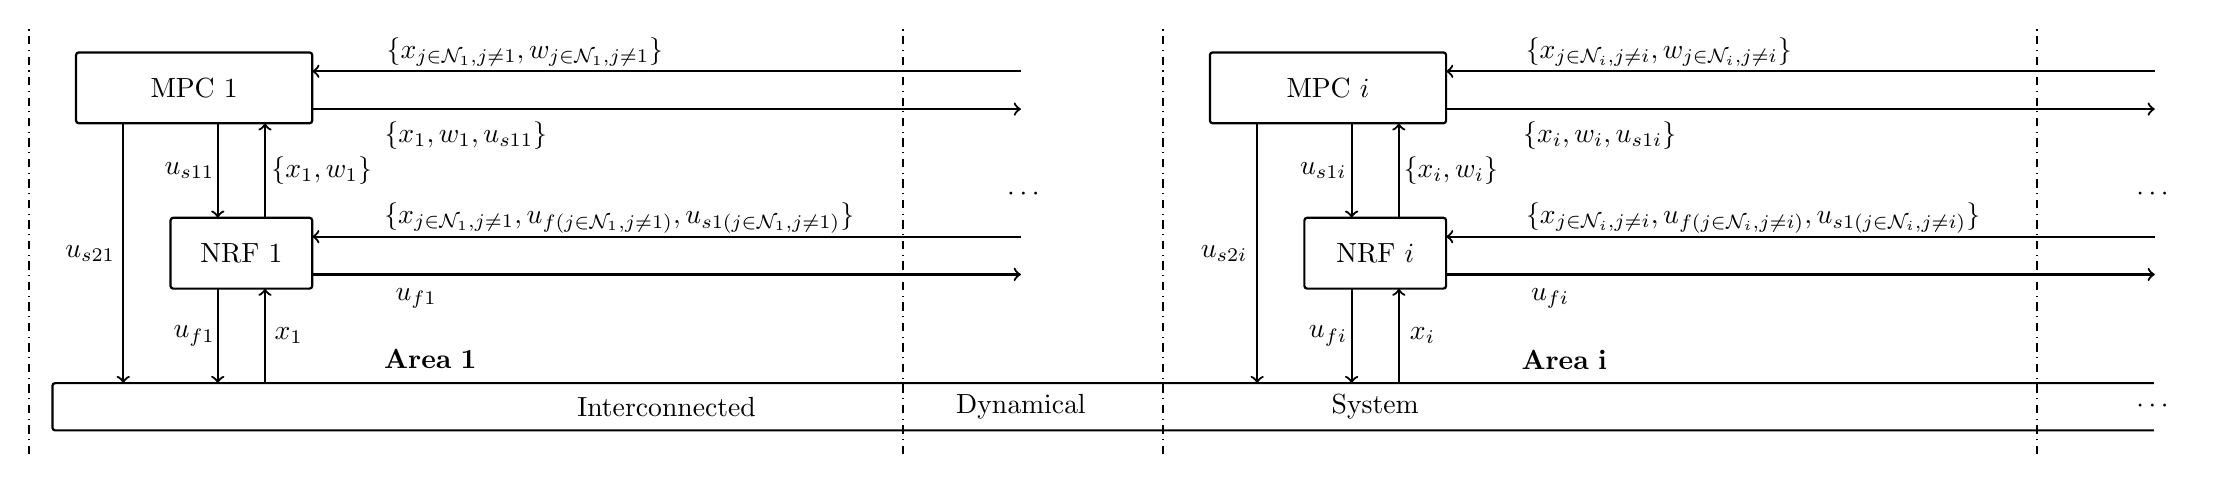
\begin{tikzpicture}[scale=0.6]
				\draw [thick,rounded corners=1]  (-15,-0.5) rectangle +(45,1);
				\draw [thick]  (-2,0)   node {Interconnected};
				\draw [thick]  (5.5,0)   node {Dynamical};
				\draw [thick]  (13,0)   node {System};
				
				\draw [thick,rounded corners=1]  (-1.5-11,2.5) rectangle +(3,1.5);
				\draw [thick]  (0-11,3.25)   node {NRF $1$};
				\node at (4-11,1) {\textbf{Area} $\mathbf 1$};
				\draw [thick,rounded corners=1]  (-3.5-11,6) rectangle +(5,1.5);
				\draw [thick]  (-1-11,6.75)   node {MPC $1$};
				\draw[->,thick] (0.5-11,0.5)--(0.5-11,2.5);
				\node at (1-11,1.5) {$x_1$};
				\draw[->,thick] (-0.5-11,2.5)--(-0.5-11,0.5);
				\node at (-1-11,1.5) {$u_{f1}$};
				\draw[->,thick] (0.5-11,4)--(0.5-11,6);
				\node at (1.7-11,5) {$\{x_1,w_1\}$};
				\draw[->,thick] (-0.5-11,6)--(-0.5-11,4);
				\node at (-1.1-11,5) {$u_{s11}$};
				\draw[->,thick] (-2.5-11,6)--(-2.5-11,0.5);
				\node at (-3.2-11,3.25) {$u_{s21}$};
				\draw[->,thick] (1.5-11,2.8)--(16.5-11,2.8);
				\node at (3.7-11,2.3) {$u_{f1}$};
				\draw[->,thick] (16.5-11,3.6)--(1.5-11,3.6);
				\node at (8-11,4) {$\{x_{j\in\mathcal{N}_1,j\neq 1},u_{f(j\in\mathcal{N}_1,j\neq 1)},u_{s1(j\in\mathcal{N}_1,j\neq 1)}\}$};
				\draw[->,thick] (1.5-11,6.3)--(16.5-11,6.3);
				\node at (4.75-11,5.75) {$\{x_1,w_1,u_{s11}\}$};
				\draw[->,thick] (16.5-11,7.1)--(1.5-11,7.1);
				\node at (6-11,7.5) {$\{x_{j\in\mathcal{N}_1,j\neq 1},w_{j\in\mathcal{N}_1,j\neq 1}\}$};
				\draw[dash dot,thick] (-4.5-11,-1)--(-4.5-11,8);
				\draw[dash dot,thick] (14-11,-1)--(14-11,8);
				
				\node at (5.6,4.5) {$\cdots$};
				
				\draw [thick,rounded corners=1]  (-1.5+13,2.5) rectangle +(3,1.5);
				\draw [thick]  (0+13,3.25)   node {NRF $i$};
				\node at (4+13,1) {\textbf{Area} $\mathbf i$};
				\draw [thick,rounded corners=1]  (-3.5+13,6) rectangle +(5,1.5);
				\draw [thick]  (-1+13,6.75)   node {MPC $i$};
				\draw[->,thick] (0.5+13,0.5)--(0.5+13,2.5);
				\node at (1+13,1.5) {$x_i$};
				\draw[->,thick] (-0.5+13,2.5)--(-0.5+13,0.5);
				\node at (-1+13,1.5) {$u_{fi}$};
				\draw[->,thick] (0.5+13,4)--(0.5+13,6);
				\node at (1.6+13,5) {$\{x_i,w_i\}$};
				\draw[->,thick] (-0.5+13,6)--(-0.5+13,4);
				\node at (-1.1+13,5) {$u_{s1i}$};
				\draw[->,thick] (-2.5+13,6)--(-2.5+13,0.5);
				\node at (-3.2+13,3.25) {$u_{s2i}$};
				\draw[->,thick] (1.5+13,2.8)--(16.5+13,2.8);
				\node at (3.7+13,2.3) {$u_{fi}$};
				\draw[->,thick] (16.5+13,3.6)--(1.5+13,3.6);
				\node at (8+13,4) {$\{x_{j\in\mathcal{N}_i,j\neq i},u_{f(j\in\mathcal{N}_i,j\neq i)},u_{s1(j\in\mathcal{N}_i,j\neq i)}\}$};
				\draw[->,thick] (1.5+13,6.3)--(16.5+13,6.3);
				\node at (4.75+13,5.75) {$\{x_i,w_i,u_{s1i}\}$};
				\draw[->,thick] (16.5+13,7.1)--(1.5+13,7.1);
				\node at (6+13,7.5) {$\{x_{j\in\mathcal{N}_i,j\neq i},w_{j\in\mathcal{N}_i,j\neq i}\}$};
				\draw[dash dot,thick] (-4.5+13,-1)--(-4.5+13,8);
				\draw[dash dot,thick] (14+13,-1)--(14+13,8);
				
				\node at (29.5,4.5) {$\cdots$};
				
				\draw [thick,color=white,fill=white]  (29.5,-0.6) rectangle +(1,1.2);
				
				\node at (29.5,0) {$\cdots$};
		\end{tikzpicture}}\vspace{-2mm}
		\caption{High-level implementation scheme depicting the proposed distributed control strategy}\vspace{-1mm}
		\label{fig:scheme}
		\hrulefill\vspace{-3mm}
	\end{figure*}
	
	
	\subsection{Distributed Networks}
	\label{subsec:distrib_part}\vspace{-3mm}
	
	The type of networks our procedure is catered towards are described by a more particular class of realizations than the ones from \eqref{eq:ss_a}-\eqref{eq:ss_b}, namely\vspace{-2mm}
	\begin{subequations}
		\begin{align}
			x[k+1] =&\ Ax[k]+B_u u[k]+B_d\,d[k],\label{eq:net_ss_a}\\
			y[k]=&\ \phantom{A}x[k]\label{eq:net_ss_b}.
		\end{align}
	\end{subequations}\phantom{ }\vspace{-9mm}
	
	Although we consider that $x$ and $u$ are completely accessible to us, in terms of measurement and actuation respectively, we do not assume that manipulating \emph{all} of this variables is possible from any one location in our physical network. This naturally separates the network into a number of $N\in\mathbb{N}$ distinct areas, with $N>1$.\vspace{-3mm}
	
	To each of the network's $N$ areas we now assign two sets of indices, which denote the entries of $x$ and $u$ that are (uniquely) accessible for measurement or actuation in that area. Without loss of generality, we assume that these indices are assigned to the sets in ascending order, since the rows and columns of the matrices expressed in \eqref{eq:net_ss_a}-\eqref{eq:net_ss_b} may be permuted at will. Therefore, each area will be represented by the pair\vspace{-2mm}
	\begin{equation}\label{eq:trip}
		\mathcal{A}_i:=(\mathcal{A}_{xi},\mathcal{A}_{ui}),\,\forall\,i\in\{1:N\},\vspace{-2mm}
	\end{equation}
	which collects the two aforementioned index sets.\vspace{-3mm}
	
	To streamline the definition of the sets given in \eqref{eq:trip}, we will provide generic expressions via the placeholder subscript $\bullet$, which stands for one of the subscripts $\{x,u\}$. Let each set contain a number of $n_{\bullet i}\in\mathbb{N}$ indices, where $n_{\bullet i}>0,\,\forall\,i\in\{1:N\}$, such that we define\vspace{-2mm}
	\begin{equation}\label{eq:net_part}
		\hspace{-1mm}\left\{\begin{split}
			\mathcal{A}_{\bullet i}:=\{\alpha_{\bullet i}+j\ \vert\ j\in1:n_{\bullet i}\},\,\forall\,i\in\{1:N\},\\
			\alpha_{\bullet 1}:=0,\, \alpha_{\bullet \ell}:=\alpha_{\bullet (\ell-1)}+n_{\bullet (\ell-1)},\,\forall\,\ell\in\{2:N\}.
		\end{split}\right.\vspace{-2mm}
	\end{equation}
	To each partition\footnote{As an example, a network with 12 states and 7 inputs could be partitioned as in \eqref{eq:trip}-\eqref{eq:net_part} via the following collection of sets $\scriptsize\begin{array}{l}
			\{(\{1:2\},\{1\}),(\{3:5\},\{2:3\}),(\{6:11\},\{4:5\}),(\{12\},\{6:7\})\}
		\end{array}$} in \eqref{eq:net_part}, we attach the selection matrix\vspace{-2mm}
	\begin{equation}\label{eq:sel_mat}
		S_{\bullet i}:=\left[\scriptsize\begin{array}{ccc}
			e_{\alpha_{\bullet i}+1}&\dots&e_{\alpha_{\bullet i}+n_{\bullet i}}
		\end{array}\right],\,\forall\,i\in\{1:N\},\vspace{-2mm}
	\end{equation}
	with which we define $x_i[k]:=S^\top_{{xi}}x[k]$, $x_{c{i}}:=S^\top_{{xi}}x_c$ and $u_i[k]:=S^\top_{{ui}}u[k]$. Once the network is partitioned, the design of our control scheme can begin.
	
	\section{The Control Architecture}\label{sec:arch}\vspace{-3mm}
	
	\subsection{Global Perspective and Objectives}\label{subsec:global_arch}\vspace{-3mm}
	
	The aim of this paper and of its companion paper \cite{part1} is to formalize the design framework of the two-layer control architecture for the interconnected dynamical system depicted in Figure~\ref{fig:scheme}. By identifying the subset of areas $\mathcal{N}_i\subseteq\{1:N\}$ which are able to transmit information to the network's $i^\text{th}$ area (and which trivially satisfy $i\in\mathcal{N}_i$), for all $i\in\{1:N\}$, the communication graph is clearly designated and the fundamental operating principle of our control scheme is the following:\vspace{-3mm}
	\begin{enumerate}
		\item[$a)$] the state-space implemented NRF subcontrollers receive network state information along with the command signals of other first layer subcontrollers from their areas' neighbourhoods, and use these values to compute the signals denoted $u_{fi}$ in Figure~\ref{fig:scheme};\smallskip
		
		\item[$b)$] the MPC subcontrollers also receive network state information along with the state variables of the NRF subcontroller implementations, denoted $w_i$ in Figure~\ref{fig:scheme}, from their areas' neighbours to compute:\smallskip
		
		\begin{enumerate}
			\item[$b1)$] the command signals denoted by $u_{s1i}$ in Figure~\ref{fig:scheme}, which \emph{are broadcast} and combined additively with the state vectors $x_i$, before the later are fed to the NRF subcontrollers;\smallskip
			
			\item[$b2)$] the command signals denoted by $u_{s2i}$ in Figure~\ref{fig:scheme}, which \emph{remain local} and are combined additively with the NRF outputs $u_{fi}$, to obtain the control signals being sent to the actuators.\vspace{-3mm}
		\end{enumerate}
	\end{enumerate}
	
	\begin{remark}
		In terms of control architecture design, it should be clear that both the first and the second layer employ feedback and feedforward components. However, their goals and their communication-based mechanisms are completely different. Where the first layer focuses on dynamical decoupling and disturbance rejection, the second layer concerns itself with constraint satisfaction and feasibility, in terms of robust control invariance.\vspace{-3mm}
	\end{remark}
	
	The architecture and design of the first layer is covered in our companion paper \cite{part1}, and this manuscript focuses on all aspects concerning the MPC-like second layer of our proposed control scheme. However, given that the MPC layer is built upon the closed-loop interconnection between the NRF layer and the network, its objectives will invariably account for the dynamics of the NRF-based subcontrollers. Thus, we briefly summarize several key concepts from \cite{part1}, before laying out the main objectives of our top-layer predictive strategies.\vspace{-3mm}
	
	
	\begin{figure}[t]
		\centering
		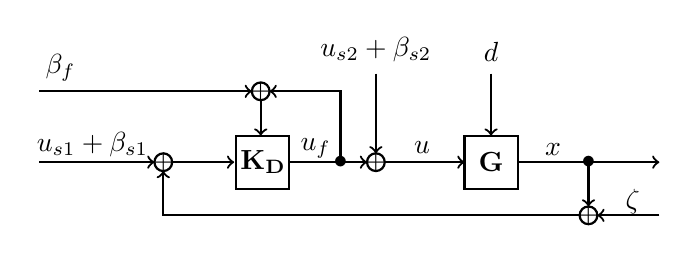
\begin{tikzpicture}[scale=0.225]
			\draw [thick] [->] (-3,0) -- (3.5,0);
			\draw [thick]  (4,0) circle(0.5);
			\draw [thick]  (4,0) node {$+$};
			\draw [thick] (3,1)   node {\bf{ }} (0,1) node {$u_{s1}+\beta_{s1}$};
			\draw [thick] [->] (4.5,0) -- (8,0);
			\draw[ thick, xshift=0.1cm]  (8,-1.5) rectangle +(3,3);
			\draw [thick] (9.5,0)   node {{$\,\mathbf{K}_{\mathbf{D}}$}} ;
			\draw [thick] [->] (11.1,0) -- (15.5,0);
			\draw [thick]  (16,0) circle(0.5cm);
			\draw [thick]  (16,0) node {$+$};
			\draw [thick] (12.6,0.8)   node {$u_f$} ;
			\draw [thick] [->] (14,0) -- (14,4)--(10,4);
			\draw [thick] (18.6,0.8)   node {$u$} ;
			\draw [thick] (14,0)   node {$\bullet$} ;
			\draw [thick]  (14.8,0.7)   node {\bf{ }};
			\draw [thick] [->] (16,5) -- (16,0.5);
			\draw [thick]  (-1.8,4)  node[anchor=south] {$\beta_f$};
			\draw [thick]  (9.5,4) circle(0.5);
			\draw [thick]  (9.5,4) node {$+$};
			\draw [thick] [->] (9.5,3.5) -- (9.5,1.5);
			\draw [thick] [->] (-3,4) -- (9,4);
			\draw [thick]  (16,5.1)  node[anchor=south] {$u_{s2}+\beta_{s2}$};
			\draw [thick] [->] (16.5,0) -- (21,0);
			\draw [thick]  (21,-1.5) rectangle +(3,3) ;
			\draw [thick]  (22.5,0)   node {{${\bf G}$}} ;
			\draw [thick]  (26,0.7)   node {$x$};
			\draw [thick] [->] (24,0) -- (32,0);
			\draw [thick] (28,0)   node {$\bullet$} ;
			\draw [thick] [->] (28,0) -- (28,-2.5);
			\draw [thick] [->] (27.5,-3) -- (4,-3)-- (4, -0.5);
			\draw [thick]  (28,-3) circle(0.5);
			\draw [thick]  (28,-3) node {$+$};
			\draw [thick] [->] (32,-3) -- (28.5,-3);
			\draw [thick]  (30.5,-2.25)  node {$\zeta$};
			\draw [thick] [->] (22.5,5) -- (22.5,1.5);
			\draw [thick]  (22.5,5.1)  node[anchor=south] {$d$};
		\end{tikzpicture}
		\caption{Feedback loop of a network's model ${\bf G}(z)$ with the NRF-based distributed implementation $\mathbf{K}_{\bf \mathbf{D}}(z)$}
		\label{fig:NRF_implem}
	\end{figure}
	
	
	\begin{figure*}
		\begin{equation}\label{eq:area_NRF}\tag{8}
			\mathbf{K}_{\mathbf{D}i}(z)=\left[\scriptsize\begin{array}{c|c}
				A_{wi}-z I_{n_{wi}} & B_{wi} \\ \hline C_{wi} & D_{wi}
			\end{array}\right]:= \left[\tiny\begin{array}{ccc|c}
				A_{r(\alpha_{ui}+1)}-z I_{n_{r(\alpha_{ui}+1)}} & & & B_{r(\alpha_{ui}+1)} \\
				& \ddots & & \vdots \\
				& & A_{r(\alpha_{ui}+n_{ui})}-z I_{n_{r(\alpha_{ui}+n_{ui})}} & B_{r(\alpha_{ui}+n_{ui})} \\ \hline 
				C_{r(\alpha_{ui}+1)} & & & O\\
				& \ddots & & \vdots\\
				& & C_{r(\alpha_{ui}+n_{ui})} & O\\
			\end{array}\right].\vspace{1mm}
		\end{equation}
		\hrulefill\vspace{-1mm}
	\end{figure*}
	
	
	
	
	\subsection{Interfacing with the First Layer}\label{subsec:interf}\vspace{-3mm}
	
	Our control architecture's first layer is implemented as depicted in Figure~\ref{fig:NRF_implem}, in which the distributed control laws are represented by the TFM
	\vspace{-3mm}
	\begin{equation}\label{eq:Kd_def}
		\mathbf{K}_{\mathbf{D}}(z):=\begin{bmatrix}
			\mathbf{K}_{\mathbf{D}1}^\top(z) & \dots & \mathbf{K}_{\mathbf{D}N}^\top(z)
		\end{bmatrix}^\top,\vspace{-3mm}
	\end{equation}
	where each $\mathbf{K}_{\mathbf{D}i}(z)=S_{ui}^\top\mathbf{K}_{\mathbf{D}}(z)$ is the TFM of the $i^\text{th}$ area's local subcontroller. Crucially, these subcontrollers are implemented via the states-space realizations given in \eqref{eq:area_NRF}, located at the top of the next page, whose component matrices (see Section 4.1 in \cite{part1} for more details) are given, for all $\ell\in\mathcal{A}_{ui}$, by 
	\vspace{-3mm}\stepcounter{equation}
	\begin{equation}\label{eq:mat_coef}
		\left\{\begin{array}{ll}
			\widetilde{A}_{r\ell}:=\tiny\begin{bmatrix}
				-a_{1\ell} &\dots& -a_{(n_{r\ell}-1)\ell}
			\end{bmatrix}^\top,& A_{r\ell}:=\ \tiny\begin{bmatrix}
				\widetilde{A}_{r\ell} & I_{n_{r\ell}-1}\\
				-a_{n_{r\ell}\ell} & O
			\end{bmatrix},\\
			B_{r\ell}:=\tiny\begin{bmatrix}
				K_{1i}^\top &\dots& K_{n_{r\ell}i}^\top
			\end{bmatrix}^\top,& C_{r\ell}:=\tiny\ \ \begin{bmatrix}
				1 & 0 & \dots & 0
			\end{bmatrix}.
		\end{array}\right.
	\end{equation}
	Henceforth, we define the orders $n_{wi}:=\textstyle\sum_{\ell=1}^{n_{ui}} n_{r\ell}$ along with $n_w:=\textstyle\sum_{i=1}^N n_{wi}$. We also denote the state vectors of the implementations from \eqref{eq:area_NRF} as $w_i[k]$ and their initial conditions as $w_{ci}\in\mathbb{R}^{n_{wi}}$. Moreover, we concatenate the latter into $w_c:=\tiny\begin{bmatrix}
		w_{c1}^\top & \dots & w_{cN}^\top
	\end{bmatrix}^\top\in\mathbb{R}^{n_w}$, which are the initial conditions of the first layer's \emph{global} implementation.\vspace{-3mm}
	
	One of the main features of this control scheme is that it is able to \emph{independently} compute the control signals of the first layer as follows\vspace{-3mm}
	\begin{equation}\label{eq:uf_implem}
		u_{fi}[k]:=S_{{ui}}^\top u_f[k] = \mathbf{K}_{\mathbf{D}i}(z)\star\tiny\begin{bmatrix}
			u_f[k]+\beta_f[k] \\ x[k]+\zeta[k]+u_{s1}[k]+\beta_{s1}[k]
		\end{bmatrix},\normalsize
	\end{equation}
	for all $i\in\{1:N\}$, while employing only information from each area's neighbourhood. Algebraically, this reduces to the fact that, for all $j\in\{1:N\}\backslash\mathcal{N}_i$, the implementations from \eqref{eq:area_NRF}-\eqref{eq:mat_coef} satisfy\vspace{-3mm}
	\begin{equation}\label{eq:dist_implem}
		\mathrm{col}_q(B_{r\ell})=O,\,\forall\,\ell\in\mathcal{A}_{ui},\,q\in\mathcal{A}_{xj}\cup(\{n_x\}\oplus\mathcal{A}_{uj}).\vspace{-3mm}
	\end{equation}
	\begin{remark}
		Although we consider the first layer's control laws to be obtained through an NRF-based framework, as in our companion paper \cite{part1}, note that any set of distributed subcontrollers implemented as in \eqref{eq:Kd_def}-\eqref{eq:dist_implem} may be employed for the procedures described in the sequel.\vspace{-3mm}
	\end{remark}
	
	The other main feature of the NRF-based layer is revealed by first introducing the exogenous signal vector\vspace{-3mm}
	\begin{equation}\label{eq:MPC_exo}
		d_s[k]:=\begin{bmatrix}
			(\zeta[k]+\beta_{s1}[k])^\top & \beta_{s2}^\top[k] & \beta_f^\top[k] & d^\top[k]
		\end{bmatrix}^\top,\vspace{-3mm}
	\end{equation}
	in which $\zeta[k]$ represents state measurement noise, $\beta_f[k]$ stands for the first layer's communication disturbance, $\beta_{s1}[k]$ and $\beta_{s2}[k]$ denote encoding errors and communication disturbance associated with the second layer's command signals and $d[k]$ is the disturbance associated directly with the networks' dynamics in \eqref{eq:net_ss_a}.\vspace{-3mm}
	
	\begin{remark}\label{rem:com}
		We assume that the communication infrastructure of our control architecture is endowed error-detecting/correcting transmission mechanisms. Therefore, all communication errors affecting transmitted information are modelled as disturbance which originates at the source of transmission, not on the receiving ends.\vspace{-3mm}
	\end{remark}
	
	By using the signal vector introduced in \eqref{eq:MPC_exo}, while also merging the MPC subcontroller's command signals from Figure~\ref{fig:scheme} into the vectors $u_{s1}[k]:=\tiny\begin{bmatrix}
		u_{s11}^\top[k] & \dots & u_{s1N}^\top[k]
	\end{bmatrix}^\top$ and $u_{s2}[k]:=\tiny\begin{bmatrix}
		u_{s21}^\top[k] & \dots & u_{s2N}^\top[k]
	\end{bmatrix}^\top$, it is possible to express the first layer's closed-loop dynamics as follows\vspace{-3mm}
	\begin{multline}\label{eq:cl_dyn}
		\scriptsize\begin{bmatrix}
			x[k]  \\  u_f[k]
		\end{bmatrix}=\mathbf{F}_{\mathbf{Q}}(z)\scriptsize\begin{bmatrix}
			I_{(n_x+n_u)} \\ O
		\end{bmatrix}\star\scriptsize\begin{bmatrix}
			u_{s1}[k] \\ u_{s2}[k]
		\end{bmatrix}+\\+\mathbf{F}_{\mathbf{Q}}(z)\star d_s[k]+\mathcal{I}_{\mathbf{Q}}[k]
		{\scriptsize\begin{bmatrix}
				x_c \\  w_c
		\end{bmatrix}}
		\,,
	\end{multline}
	\phantom{}
	
	\vspace{-9mm}
	where $\mathbf{F}_{\mathbf{Q}}(z)$ is a strictly proper ($\lim_{z\rightarrow\infty}\mathbf{F}_{\mathbf{Q}}(z)=O$) TFM which models the closed-loop's response to exogenous inputs, and $\mathcal{I}_{\mathbf{Q}}[k]$ is a time-varying matrix which governs the closed-loop system's evolution with respect to initial conditions. The main result of our companion paper \cite{part1} shows that $\mathbf{F}_{\mathbf{Q}}(z)$ and $\mathcal{I}_{\mathbf{Q}}[k]$ are easily tunable via a freely chosen $\mathbf{Q}$-parameter (hence, the employed notation), thus enabling the \emph{complete design} of the first layer's closed-loop response. It is with respect to the dynamics given in \eqref{eq:cl_dyn} that we formulate both the objectives and the design procedure of our second layer.\vspace{-3mm}
	
	
	
	
	
	\subsection{Objectives of the MPC Layer}\label{subsec:MPC_obj}\vspace{-3mm}
	
	
	
	Given the high-level functioning principles described in Section~\ref{subsec:global_arch} and the closed-loop dynamics summarized in Section~\ref{subsec:interf}, our MPC-based second layer must simulta-
	\newpage
	neously achieve the following objectives:\vspace{-2mm}
	\begin{enumerate}
		\item[$\mathrm I)$] it employs tractable and area-based prediction models, which completely capture the local behaviour of the dynamics given in \eqref{eq:cl_dyn} (Section~\ref{sec:transform});\smallskip
		
		\item[$\mathrm{II})$] it formulates and manages all of its constraints in a distributed manner, by adapting set-theoretical techniques \cite{STMC} in accordance with the area partitioning from \eqref{eq:trip}-\eqref{eq:net_part}  (Section~\ref{sec:MPC_des});\smallskip
		
		\item[$\mathrm{III})$] it admits a formulation based upon \emph{receding horizon optimization} (see, for example, Chapter 1 in \cite{RMD}) which regulates only \emph{local} variables $\{x_i,u_{fi}\}$, but ensures \emph{global} constraint satisfaction and recursive feasibility (Section~\ref{sec:MPC_imp});\vspace{-2mm}
		
	\end{enumerate}
	
	The remainder of this paper is dedicated to presenting the solutions to these design challenges.\vspace{-3mm}
	
	\section{Obtaining an MPC-Oriented Formulation}\vspace{-3mm}
	\label{sec:transform}
	
	
	
	
	\subsection{Nominal Area-based Prediction Models}\vspace{-3mm}
	
	In order to formulate tractable prediction models for our architecture's second layer, we need to account for the state variables of the implementations from \eqref{eq:area_NRF}. Thus, aside from the $x$ and $u$ subscripts appearing in \eqref{eq:net_part}-\eqref{eq:sel_mat}, we introduce the additional subscript $w$, in order to refer to the state vector of each area's NRF subcontroller, and we extend the index collection defined originally in \eqref{eq:trip} to $\mathcal{A}_i:=(\mathcal{A}_{xi},\mathcal{A}_{ui},\mathcal{A}_{wi}),\,\forall\,i\in\{1:N\}$.\vspace{-3mm} 
	
	We begin our reformulation of the first-layer's closed-loop dynamics by pointing out that, due to the fact that the TFM $\mathbf{F}_{\mathbf{Q}}(z)$ from \eqref{eq:cl_dyn} is strictly proper, it is always possible to obtain state-space realizations of type\vspace{-3mm}
	\begin{equation}\label{eq:disc_real}
		\left[\tiny\begin{array}{cc}
			S^\top_{{xi}} & O \\\hdashline
			O & S^\top_{{ui}}
		\end{array}\right]\mathbf{F}_{\mathbf{Q}}(z)\left[\tiny\begin{array}{c:c}
			S_{{xi}} & O\\O & S_{{ui}}\\ O & O
		\end{array}\right]=\left[\tiny\begin{array}{c|c:c}
			A_{si}-zI_{n_{si}} & B_{s1i} & B_{s2i}\\\hline C_{xi} & O & O\\\hdashline C_{ui} & O & O
		\end{array}\right],
	\end{equation}
	for all $i\in\{1:N\}$. By defining now $Z_i:=\mathrm{diag}(S_{xi},S_{ui})$ along with ${Z}_{ci}:=\mathrm{diag}(S_{xi},S_{wi})$, we employ the realizations from \eqref{eq:disc_real} to describe the MPC-oriented area model of the $i^\text{th}$ area, which can be expressed as\vspace{-2mm}
	\begin{subequations}
		\begin{align}\label{eq:disc_cl_dyn_a}
			\xi_i[k+1] =A_{si} \xi_i[k] + &\ B_{s1i} u_{s1i}[k]+B_{s2i} u_{s2i}[k],\\
			\label{eq:disc_cl_dyn_b}
			x_i[k] =C_{xi} \xi_i[k] + &\ (\psi_{x i}[k] + \theta_{x i}[k] + \delta_{x i}[k]),\\
			u_{fi}[k] =C_{ui} \xi_i[k] + &\ (\psi_{ui}[k] + \theta_{ui}[k] + \delta_{ui}[k]),\label{eq:disc_cl_dyn_c}\\
			\label{eq:disc_cl_dyn_d}
			&\hspace{-22mm}k\in\mathbb{N},\ k\geq k_0,\ \xi_i[k_0]=O,\,\forall\,i\in\{1:N\},
		\end{align}
	\end{subequations}
	\phantom{}
	
	\vspace{-10mm}
	where we have that\vspace{-2mm}
	\begin{enumerate}
		\item[a)] $\xi_i[k]$ is the state vector of the realization obtained in \eqref{eq:disc_real} and which \emph{always} has zero initial conditions at initial time $k_0$ (recall the identity from \eqref{eq:forced_resp});\bigskip
		
		\item[b)] the contribution of exogenous disturbance to the area dynamics is given by \vspace{-3mm}
	\end{enumerate}
	\begin{equation}\label{eq:disc_cl_dyn_1}
		\left\{
		\begin{split}
			\psi_i[k]:=&\ Z_i^\top\mathbf{F}_{\mathbf{Q}}(z)\star d_s[k],\\
			\psi_{x i}[k]:=&\ \tiny\begin{bmatrix}
				I_{n_{xi}} & O
			\end{bmatrix}\psi_i[k],\ 
			\psi_{ui}[k]:=\ \tiny\begin{bmatrix}
				O & I_{n_{ui}}
			\end{bmatrix}\psi_i[k],
		\end{split}
		\right.\vspace{-3mm}\hspace{-1mm}
	\end{equation}
	\begin{enumerate}
		\item[c)] the contribution of the \emph{neighbouring} areas' initial conditions to the area dynamics is given by\vspace{-3mm}
	\end{enumerate}
	\begin{equation}\label{eq:disc_cl_dyn_2}
		\left\{\begin{split}
			&\theta_i[k]:=\textstyle\sum_{j\in\mathcal{N}_i}Z_i^\top \mathcal{I}_{\mathbf{Q}}[k]Z_{cj}\tiny\begin{bmatrix}
				x_{cj}\\w_{cj}
			\end{bmatrix},\normalsize\\
			&\theta_{x i}[k]:=\tiny\begin{bmatrix}
				I_{n_{xi}} &O
			\end{bmatrix}\theta_i[k],\ \theta_{ui}[k]:=\tiny\begin{bmatrix}
				O & I_{n_{ui}}
			\end{bmatrix}\theta_i[k],
		\end{split}
		\right.\vspace{-3mm}
	\end{equation}
	\begin{enumerate}
		\item[d)] the \emph{residual} contributions of initial conditions from outside of the $i^\text{th}$ area's neighbourhood and of cross-coupling with other areas' MPC subcontrollers is\vspace{-3mm}
	\end{enumerate}\begin{equation}\label{eq:disc_cl_dyn_3}
		\hspace{-2mm}\left\{\begin{split}
			&\delta_i[k]:=\hspace{-2mm}\sum_{j\in\{1:N\}\backslash\{i\}}\hspace{-2mm}Z_i^\top\mathbf{F}_{\mathbf{Q}}(z)\tiny\begin{bmatrix}
				Z_j\\O
			\end{bmatrix}\star\begin{bmatrix}
				u_{s1j}[k] \\ u_{s2j}[k]
			\end{bmatrix}+\\&\qquad\qquad\quad\,+\sum_{j\in\{1:N\}\backslash\mathcal{N}_i}Z_i^\top \mathcal{I}_{\mathbf{Q}}[k]Z_{cj}\tiny\begin{bmatrix}
				x_{cj}\\w_{cj}
			\end{bmatrix},\\
			&\delta_{x i}[k]:=\tiny\begin{bmatrix}
				I_{n_{xi}} & O
			\end{bmatrix}\delta_i[k],\ \delta_{ui}[k]:=\tiny\begin{bmatrix}
				O & I_{n_{ui}}
			\end{bmatrix}\delta_i[k],
		\end{split}\right.\vspace{-3mm}
		\normalsize
	\end{equation}
	
	The signals from \eqref{eq:disc_cl_dyn_1}-\eqref{eq:disc_cl_dyn_3} separate naturally into two classes, in the form of information that is:\vspace{-3mm}
	\begin{enumerate}
		\item[$i)$]  \emph{available} to a second layer subcontroller, represented by $\theta_{xi}[k]$ and $\theta_{ui}[k]$;\smallskip
		
		\item[$ii)$] \emph{unavailable} to a second layer subcontroller, represented by $(\psi_{xi}[k]+\delta_{xi}[k])$ and $(\psi_{ui}[k]+\delta_{ui}[k])$.\vspace{-3mm}
	\end{enumerate}
	
	\begin{remark}\label{rem:decup}
		The quantities described in \eqref{eq:disc_cl_dyn_3} are called \emph{residual} due to the fact that it is the primary goal of the first layer to attenuate the effect that these signals have on the area dynamics from \eqref{eq:disc_cl_dyn_a}-\eqref{eq:disc_cl_dyn_d}. Indeed, since these terms represent the contribution of all the variables which are not available (in terms of measurement or prediction) to the $i^\text{th}$ area, the only sensible recourse is to minimize their influence (see Section 5 in \cite{part1}).  \vspace{-3mm}
	\end{remark}
	
	Thus, each subcontroller must employ the information that is encoded in the signals from \eqref{eq:disc_cl_dyn_2} to compute a pair of commands $u_{s1i}[k]$ and $u_{s2i}[k]$ which robustly account for the effects of the signals from \eqref{eq:disc_cl_dyn_1} and \eqref{eq:disc_cl_dyn_3}. Yet, before translating this objective into a set-theoretical formulation, we investigate the effect of \emph{unreliable measurements} for $x_c$ and $w_c$ in the distributed setting.\vspace{-3mm}
	
	\subsection{Accounting for Inaccurate Initial Conditions}\label{subsec:ci_dist}\vspace{-3mm}
	
	Given some pre-specified set $\mathcal{V}\subseteq\mathbb{R}^{n_x+n_w}$, we consider the additively disturbed initial conditions defined as\vspace{-3mm}
	\begin{equation}\label{eq:noise_init}
		\tiny\begin{bmatrix}
			\widetilde{x}_c \\ \widetilde{w}_{c}
		\end{bmatrix}:=\tiny\begin{bmatrix}
			{x}_c+\nu_x \\{w}_{c}+\nu_w
		\end{bmatrix},\quad 	\tiny\begin{bmatrix}
			\widetilde{x}_{c{i}} \\ \widetilde{w}_{ci}
		\end{bmatrix}:=\tiny\begin{bmatrix}
			{x}_{ci}+S^\top_{{xi}}\nu_x \\ {w}_{ci}+S^\top_{{wi}}\nu_w
		\end{bmatrix},\normalsize\vspace{-3mm}
	\end{equation}
	for any index $i\in\{1:N\}$ along with any $\tiny\begin{bmatrix}
		\nu_x^\top \ \,\nu_w^\top
	\end{bmatrix}^\top\in\mathcal{V}$.\vspace{-3mm}
	\begin{remark}\label{rem:ci_dist_cause}
		In light of the arguments made in Remark~\ref{rem:com}, notice that the type of disturbance discussed in this section can always be modelled as in \eqref{eq:noise_init}. Practical causes for these unwanted terms include noisy measurement of the network's state variables and faulty reading of the NRF-based controller's state vector.\vspace{-3mm}
	\end{remark}
	
	The main consequence of taking into account these terms is that the prediction models from \eqref{eq:disc_cl_dyn_b}-\eqref{eq:disc_cl_dyn_c} become\vspace{-3mm}
	\begin{subequations}
		\begin{align}
			\label{eq:noise_pert_1}
			\widetilde x_i[k] =&\ C_{xi} \xi_i[k] + (\psi_{x i}[k] + \widetilde\theta_{x i}[k] + \widetilde\delta_{x i}[k]),\\
			\widetilde u_{fi}[k] =&\ C_{ui} \xi_i[k] + (\psi_{u i}[k] + \widetilde\theta_{u i}[k] + \widetilde\delta_{u i}[k]),\label{eq:noise_pert_2}
		\end{align}
	\end{subequations}
	\phantom{}
	
	\vspace{-10mm}
	when considering the noise-affected initial conditions introduced in \eqref{eq:noise_init} instead of the real ones, where\vspace{-3mm}
	\begin{equation}\label{eq:disc_cl_dyn_2p}
		\hspace{-2mm}\left\{\begin{split}
			\widetilde \theta_i[k]:=&\ \theta_i[k] + \sum_{j\in\mathcal{N}_i}Z_i^\top \mathcal{I}_{\mathbf{Q}}[k]Z_{cj}\tiny\begin{bmatrix}
				S^\top_{{xj}}\nu_x \\ S^\top_{{wj}}\nu_w
			\end{bmatrix},\\
			\widetilde \theta_{x i}[k]:=&\ \tiny\begin{bmatrix}
				I_{n_{xi}} & O
			\end{bmatrix}\widetilde \theta_i[k],\ 
			\widetilde \theta_{ui}[k]:=\ \tiny\begin{bmatrix}
				O & I_{n_{ui}}
			\end{bmatrix}\widetilde \theta_i[k],
		\end{split}
		\right.\hspace{-3mm}\vspace{-3mm}
	\end{equation}
	along with\vspace{-3mm}
	\begin{equation}\label{eq:disc_cl_dyn_3p}
		\hspace{-2mm}\left\{\begin{split}
			\widetilde \delta_i[k]:=&\ \delta_i[k]+\sum_{j\in\{1:N\}\backslash\mathcal{N}_i}Z_i^\top \mathcal{I}_{\mathbf{Q}}[k]Z_{cj}\tiny\begin{bmatrix}
				S^\top_{{xj}}\nu_x \\ S^\top_{{wj}}\nu_w
			\end{bmatrix},\\
			\widetilde \delta_{x i}[k]:=&\ \tiny\begin{bmatrix}
				I_{n_{xi}} & O
			\end{bmatrix}\widetilde \delta_i[k],\ 
			\widetilde \delta_{ui}[k]:=\ \tiny\begin{bmatrix}
				O & I_{n_{ui}}
			\end{bmatrix}\widetilde \delta_i[k],
		\end{split}\right.\hspace{-2mm}\vspace{-3mm}
		\normalsize
	\end{equation}
	represent the noise-affected versions of the signals from \eqref{eq:disc_cl_dyn_2} and \eqref{eq:disc_cl_dyn_3}, respectively, for all $i\in\{1:N\}$.\vspace{-3mm}
	
	\subsection{Connecting the Augmented Prediction Models to the Nominal Ones}\label{subsec:aug_pred}\vspace{-3mm}
	
	Since the vector $\tiny\begin{bmatrix}
		\nu_x^\top & \nu_w^\top
	\end{bmatrix}^\top$ cannot be determined \emph{a priori}, our MPC-based subcontrollers will have to make use of the initial conditions in \eqref{eq:noise_init} instead of the real ones. Consequently, our control policies will employ the prediction models affected by additive disturbance \eqref{eq:noise_pert_1}-\eqref{eq:noise_pert_2}, instead of the ones given in \eqref{eq:disc_cl_dyn_b}-\eqref{eq:disc_cl_dyn_c}. However, a straightforward computation yields the fact that the original area dynamics, given by the identities obtained in \eqref{eq:disc_cl_dyn_b}-\eqref{eq:disc_cl_dyn_c}, can be retrieved from \eqref{eq:noise_pert_1}-\eqref{eq:noise_pert_2} via\vspace{-3mm}
	\begin{equation}\label{eq:noise_pert_3}
		x_i[k]=\widetilde x_i[k]-\eta_{x i}[k],\quad u_{fi}[k]=\widetilde{u}_{fi}[k]-\eta_{ui}[k],\vspace{-3mm}
	\end{equation}
	for all $i\in\{1:N\}$, where $\eta_{x i}[k]$ and $\eta_{ui}[k]$ are defined as\vspace{-3mm}
	\begin{equation}\label{eq:disc_cl_dyn_4}
		\left\{\begin{split}
			\eta_i[k]:=&\ \textstyle\sum_{j=1}^{N}Z_i^\top \mathcal{I}_{\mathbf{Q}}[k]Z_{cj}\tiny\begin{bmatrix}
				S^\top_{{xj}}\nu_x \\ S^\top_{{wj}}\nu_w
			\end{bmatrix},\\
			\eta_{x i}[k]:=&\ \tiny\begin{bmatrix}
				I_{n_{xi}} & O
			\end{bmatrix}\eta_i[k],\ 
			\eta_{ui}[k]:=\ \tiny\begin{bmatrix}
				O & I_{n_{ui}}
			\end{bmatrix}\eta_i[k].
		\end{split}\right.
		\normalsize\vspace{-3mm}
	\end{equation}
	Having obtained the area-based prediction models in \eqref{eq:disc_cl_dyn_a}-\eqref{eq:disc_cl_dyn_d} and having augmented them as in \eqref{eq:noise_pert_1}-\eqref{eq:noise_pert_2}, it follows that objective $I)$ from Section~\ref{subsec:MPC_obj} has been fully addressed. We now proceed to discuss constraint formulation in the distributed setting, and the means by which the identities from \eqref{eq:noise_pert_3} can be employed to ensure constraint satisfaction (in the presence of unreliable initial conditions) for the variables in \eqref{eq:disc_cl_dyn_b}-\eqref{eq:disc_cl_dyn_c}.
	\vspace{-3mm}
	
	
	\section{Constraints in the Distributed Setting}\vspace{-3mm}
	\label{sec:MPC_des}
	
	The first step in breaking down the second layer's distributed synthesis problem into locally solvable subproblems is to assign independent control objectives to each of the network's $N$ areas. Therefore, if the goal is to ensure that the signal vectors $x$ and $u$ are constrained (for all instances of time, relative to an initial moment $k_0$) to a pair of sets $\mathcal{X}\subseteq\mathbb{R}^{n_x}$ and $\mathcal{U}\subseteq\mathbb{R}^{n_u}$, respectively, then our procedure must begin by defining the pairs of sets $(\mathcal{X}_i,\mathcal{U}_i)$, with $i\in\{1:N\}$, such that\vspace{-3mm}
	\begin{equation}\label{eq:set_equiv}
		\left\{
		\begin{split}
			x[k]\in\mathcal{X}&\Longleftrightarrow x_i[k]\in\mathcal{X}_i,\,\forall\,i\in\{1:N\},\\
			u[k]\in\mathcal{U}&\Longleftrightarrow u_i[k]\in\mathcal{U}_i,\,\forall\,i\in\{1:N\}.
		\end{split}
		\right.\vspace{-3mm}
	\end{equation}\newpage
	
	\begin{remark}\label{rem:set_decomp}
		The assumption that the pair $(\mathcal{X},\mathcal{U})$ can be decomposed as in \eqref{eq:set_equiv} is not only required, when attempting to break down the global problem into any configuration of local subproblems, but it is also a mild one (see its equivalent counterpart in \cite{DMPC1}-\cite{DMPC2}). Indeed, the conditions located on the left-hand side of \eqref{eq:set_equiv} are often represented (in practice) by box constraints, for which the aforementioned decomposition may always be performed.\vspace{-3mm}
	\end{remark}
	
	The aim of the subcontrollers which form the second layer (recall Figure~\ref{fig:scheme}) is to ensure the \emph{global}, left-hand side inclusions from \eqref{eq:set_equiv} by independently satisfying the \emph{local} ones, on the right-hand side of \eqref{eq:set_equiv}. With respect to the components of the closed-loop dynamics from \eqref{eq:cl_dyn}, this problem can be broken down into five subproblems:\vspace{-3mm}
	\begin{enumerate}
		\item[$i)$] accounting (in a set-theoretical framework) for the effect of the exogenous disturbance from \eqref{eq:MPC_exo};\smallskip
		
		\item[$ii)$] translating the command-related objectives from \eqref{eq:set_equiv} into first layer command constraints;\smallskip
		
		\item[$iii)$] linking command constraints to the state variables of the implementations from \eqref{eq:area_NRF};\smallskip
		
		\item[$iv)$] accounting for the inaccurate measurements modelled in \eqref{eq:noise_init};\smallskip
		
		\item[$v)$] accounting for area cross-coupling.\vspace{-3mm}
	\end{enumerate}
	We now proceed to tackle each of these subproblems, in the order in which they are indicated.\vspace{-3mm}
	
	\subsection{Placing Constraints on Exogenous Disturbance}\vspace{-3mm}
	
	We begin by addressing the components of the signal vector from \eqref{eq:MPC_exo}. Recalling the measurement noise set from \eqref{eq:noise_init} and the arguments made in Remark~\ref{rem:ci_dist_cause}, we begin by considering that $\zeta[k]\in\tiny\begin{bmatrix}
		I_n & O
	\end{bmatrix}\mathcal{V}$. We contain the rest of the exogenous signals from \eqref{eq:MPC_exo} by introducing\vspace{-3mm}
	\begin{equation}\label{eq:dist_sets}
		\left\{\hspace{-1mm}
		\scriptsize\begin{array}{ll}
			\mathcal D_{d}\subseteq\mathbb{R}^{n_d}\,\text{s.t. }d[k]\in \mathcal D_{d},
			&\mathcal D_{\beta_f}\subseteq\mathbb{R}^{n_u}\,\text{s.t. }\beta_{f}[k]\in \mathcal D_{\beta_f},\\
			\mathcal D_{\beta_{s1}}\subseteq\mathbb{R}^{n_x}\,\text{s.t. }\beta_{s1}[k]\in \mathcal D_{\beta_{s1}},
			&\mathcal D_{\beta_{s2}}\subseteq\mathbb{R}^{n_x}\,\text{s.t. }\beta_{s2}[k]\in \mathcal D_{\beta_{s2}}.
		\end{array}
		\right.
	\end{equation}
	By doing so, it becomes possible to construct the set $
	\mathcal{D}_s\subseteq\mathbb{R}^{2n_u+n_x+n_d}$ which satisfies $d_s[k]\in\mathcal{D}_s$ and which, in tandem with the expressions from \eqref{eq:disc_cl_dyn_1}, enables us to compute the sets containing the effects of $d_s[k]$, with $k\geq k_0$, on each area's dynamics, henceforth denoted as\vspace{-3mm}
	\begin{equation}\label{eq:pert_sets}
		\hspace{-2mm}\left\{
		\begin{split}
			\Psi_{x i t}\subseteq\mathbb{R}^{n_{xi}}\text{ s.t. }\psi_{x i}[k_0+t]\in\Psi_{x i t},\,\forall\,d_s[k]\in\mathcal{D}_s,\\
			\Psi_{u i t}\subseteq\mathbb{R}^{n_{ui}}\text{ s.t. }\psi_{ui}[k_0+t]\in\Psi_{u i t},\,\forall\,d_s[k]\in\mathcal{D}_s.
		\end{split}
		\right.\hspace{-1mm}\vspace{-3mm}
	\end{equation}
	Moving onward, we address the variables associated with the first layer subcontrollers and their implementations.\vspace{-3mm}
	
	\subsection{Placing Constraints on First Layer Commands}\vspace{-3mm}
	
	A cursory inspection of Figure~\ref{fig:NRF_implem} reveals the identity\vspace{-3mm}
	\begin{equation}\label{eq:app_cmd}
		u_i[k]=u_{fi}[k]+u_{s2i}[k]+S^\top_{{ui}}\beta_{s2}[k],\,\forall\,i\in\{1:N\}.\vspace{-3mm}
	\end{equation}
	Given the state dynamics obtained in Section~\ref{sec:transform}, the problem of constraining the command signals sent to the network reduces to judiciously constraining the control effort of both the first and the second layer. Thus, for each area, we choose a pair of sets \vspace{-3mm}
	\begin{subequations}
		\begin{align}\label{eq:cmd_sets_1}
			&{\mathcal{U}}_{s1i}\subseteq\mathbb{R}^{n_{xi}}\text{ s.t. }u_{s1i}[k]\in{\mathcal{U}}_{s1i},\,\forall\,i\in\{1:N\},\\
			&{\mathcal{U}}_{s2i}\subseteq\mathbb{R}^{n_{ui}}\text{ s.t. }u_{s2i}[k]\in{\mathcal{U}}_{s2i},\,\forall\,i\in\{1:N\}.\label{eq:cmd_sets_2}
		\end{align}
	\end{subequations}\newpage
	
	and we employ the ones from \eqref{eq:cmd_sets_2} in order to compute\vspace{-3mm}
	\begin{equation}\label{eq:NRF_cmd_sets}
		{\mathcal{U}}_{fi}:=\mathcal{U}_i\ominus(\,\mathcal{U}_{s2i}\oplus(S^\top_{{ui}}\mathcal{D}_{\beta_{s2}})),\,\forall\,i\in\{1:N\}.\vspace{-3mm}
	\end{equation}
	Notice that we have $u_{fi}[k]\in{\mathcal{U}}_{fi}\Longrightarrow u_{i}[k]\in\mathcal{U}_{i}$, which allows us to translate the objectives given in \eqref{eq:set_equiv} to the output vectors of our area dynamics from \eqref{eq:disc_cl_dyn_a}-\eqref{eq:disc_cl_dyn_d}. \vspace{-3mm}
	
	%{\color{red} To prevent conservatism in computing the sets from \eqref{eq:NRF_cmd_sets}, the operation should involve only boxes.}
	
	\begin{remark}\label{rem:cmd_sets}
		The sets given in \eqref{eq:cmd_sets_1}-\eqref{eq:cmd_sets_2} are the \emph{main design parameters} of the second layer and they can be assimilated with the extent to which the second layer is permitted to interfere in the dynamics of the first layer's closed-loop system, in order to ensure that \eqref{eq:set_equiv} is satisfied. The manner in which these sets may be chosen and its associated trade-off will be discussed in the sequel.\vspace{-3mm}
	\end{remark}
	
	\subsection{Placing Constraints on First Layer States}\vspace{-3mm}
	
	Since the initial conditions of the first layer's state-space implementation explicitly impact the signals located on the left-hand side of \eqref{eq:cl_dyn}, it follows that the state vectors of the NRF-based subcontrollers from \eqref{eq:area_NRF} should also possess a state-based description, which will be used to ensure the satisfaction of the inclusions in \eqref{eq:set_equiv}.\vspace{-3mm}
	
	We begin by inspecting the distinctive structure of the matrices which make up the realizations from \eqref{eq:area_NRF}. The latter enable us to naturally partition each of the state vectors belonging to the first layer subcontrollers into $w_i[k]=\tiny\begin{bmatrix}
		w_{r(\alpha_{ui}+1)}^\top[k] & \dots & w_{r(\alpha_{ui}+n_{ui})}^\top[k]
	\end{bmatrix}$, in which the vectors $w_{r\ell}[k]$ have $n_{r\ell}$ rows for all $\ell\in\{1:n_u\}$, \emph{i.e.}, the same as the matrices $A_{r\ell}$ and $B_{r\ell}$ from \eqref{eq:mat_coef}. Recalling \eqref{eq:mat_coef}, the key observation which underpins the entire mathematical mechanism presented in this section is the fact that
	$\mathrm{row}_\ell(u_f[k])=C_{r\ell}w_{r\ell}[k]=\mathrm{row}_1(w_{r\ell}[k])$, for all $\ell\in\{1:n_u\}$. Thus, our current objective becomes apparent: we aim to employ the bounds placed upon the partitions of $u_f[k]$ in order to satisfy further set inclusions with respect to $w_{r\ell}[k]$, in a distributed manner.\vspace{-3mm}
	
	
	In order to state the main result of this section, we introduce the sets ${\mathcal{W}}_{\ell1}\subseteq\mathbb{R}$, with $\ell\in\{1:n_u\}$, which satisfy\vspace{-3mm}
	\begin{equation}\label{eq:Wi_sets}
		\mathrm{row}_\ell({u}_{f}[k])\in \mathcal{W}_{\ell1},\,\forall\,\ell\in\mathcal{A}_{ui} \Longrightarrow  u_{fi}[k]\in{\mathcal{U}}_{fi},\vspace{-3mm}
	\end{equation}
	for all $i\in\{1:N\}$. The following result employs the newly introduced sets in order to constrain the state variables of the first layer subcontrollers.\vspace{-3mm}
	
	\begin{proposition}\label{prop:NRF_state_manip}
		Let the first layer subcontrollers be implemented as in \eqref{eq:Kd_def}-\eqref{eq:dist_implem}. For each $i\in\{1:N\}$, define ${Z}_{ri}:=\mathrm{diag}(S_{ui},S_{xi})$ and the sets from \eqref{eq:feedback_set} and \eqref{eq:NRF_state_sets_a}-\eqref{eq:NRF_state_sets_b}, located at the top of the next page. Assume that:\vspace{-3mm}
		\begin{enumerate}
			\item[$A1)$] the inclusions given in \eqref{eq:dist_sets}, \eqref{eq:cmd_sets_1}-\eqref{eq:cmd_sets_2} and \eqref{eq:feedback_set} hold for $k=k_0$,
			
			\item[$A2)$] $\mathrm{row}_j(w_{r\ell}[k_0])\in\mathcal{W}_{\ell j},\,\forall\,\ell\in\mathcal{A}_{ui},\,j\in\{1:n_{r\ell}\}$,
			
			\item[$A3)$] $\mathrm{row}_\ell({u}_{f}[k_0+1])\in \mathcal{W}_{\ell1},\,\forall\,\ell\in\mathcal{A}_{ui},\,i\in\{1:N\}$,\vspace{-3mm}
		\end{enumerate}
		given some $k_0\in\mathbb{N}$. Then, $\forall\,i\in\{1:N\}$, we have that:\vspace{-3mm}
		\begin{enumerate}
			\item[$i)$] $\mathrm{row}_j(w_{r\ell}[k_0+1])\in\mathcal{W}_{\ell 1},\,\forall\,\ell\in\mathcal{A}_{ui},\,j\in\{1:n_{r\ell}\}$;
			
			\item[$ii)$] $u_{i}[k_0]\in{\mathcal{U}}_{i}$.\vspace{-6mm}
		\end{enumerate}
	\end{proposition}
	\begin{pf}
		See Appendix~\ref{app:proofs}.\vspace{-6mm}
	\end{pf}
	
	\begin{figure*}
		\begin{multline}\label{eq:feedback_set}
			{\mathcal{D}}_{wi}\subseteq\mathbb{R}^{n_{ui}+n_{xi}}\text{ s.t. }
			\tiny\begin{bmatrix}
				u_{fi}[k]+S^\top_{{ui}}\beta_f[k]\\  x_i[k]+S^\top_{{xi}}\zeta[k]+u_{s1i}[k]+S^\top_{{xi}}\beta_{s1}[k]
			\end{bmatrix}\in{\mathcal{D}}_{wi},\\
			\forall\ 
			u_{fi}[k]\in{\mathcal{U}}_{fi},\ 
			(S^\top_{{ui}}\beta_f[k])\in S^\top_{{ui}}\mathcal{D}_{\beta_f},\ 
			x_{i}[k]\in{\mathcal{X}}_{i},
			(S^\top_{{xi}}\zeta[k])\in\tiny\begin{bmatrix}
				S^\top_{{xi}}\ O
			\end{bmatrix}\mathcal{V},\ u_{s1i}[k]\in\mathcal{U}_{s1i},\  
			(S^\top_{{xi}}\beta_{s1}[k])\in S^\top_{{ui}}\mathcal{D}_{\beta_{s1}}.
		\end{multline}\vspace{-3mm}
		\phantom{ }
		
		\vspace{-5mm}
		\hrulefill\vspace{-2mm}
		\begin{subequations}
			\begin{align}\label{eq:NRF_state_sets_a}
				\mathcal{W}_{\ell n_{r\ell}}:=&\ (-a_{n_{r\ell}\ell})\mathcal{W}_{\ell 1} \oplus\left(\textstyle\bigoplus_{p\in\mathcal{N}_i}\left(K_{n_{r\ell}\ell}Z_{rp}Z_{rp}^\top\right){\mathcal{D}}_{wp}\right),\,\forall\ \ell\in\mathcal{A}_{ui},\\
				\mathcal{W}_{\ell j}:=&\ (-a_{j\ell})\mathcal{W}_{\ell 1} \oplus\mathcal{W}_{\ell (j+1)}\oplus\left(\textstyle\bigoplus_{p\in\mathcal{N}_i}\left(K_{j\ell}Z_{rp}Z_{rp}^\top\right){\mathcal{D}}_{wp}\right),\,\forall\,\ell\in\mathcal{A}_{ui},\,j\in\{2:n_{r\ell}-1\}.\label{eq:NRF_state_sets_b}
			\end{align}
		\end{subequations}\vspace{-2mm}
		\phantom{ }
		
		\vspace{-5mm}
		\hrulefill\vspace{-1mm}
	\end{figure*}
	
	
	\begin{remark}
		Note that the $i^\text{th}$ area's sets from \eqref{eq:NRF_state_sets_a}-\eqref{eq:NRF_state_sets_b} are computed efficiently, using only for those indices belonging to $\mathcal{N}_i$. This is owed to the sparsity structure displayed in \eqref{eq:dist_implem}, which serves to incentivise the synthesis of sparse control laws for the first layer (see \cite{part1}).\vspace{-3mm}
	\end{remark}
	
	The result formalized via Proposition~\ref{prop:NRF_state_manip} will prove instrumental in guaranteeing the recursive feasibility of the second layer and, in retrospect, the choice to impose constraints upon $u_{fi}[k]$, instead of the $u_i[k]$ vectors in \eqref{eq:set_equiv}, becomes justified. Not only do the \emph{specialized implementations} presented in \eqref{eq:area_NRF} allow us to construct set-based descriptions \eqref{eq:NRF_state_sets_a}-\eqref{eq:NRF_state_sets_b} for the states belonging to the first layer implementations, but they also enable us to \emph{explicitly link} the aforementioned sets to the second layer's design objectives. By eliminating \emph{the need to individually select} each of these sets (which is an intricate and highly empirical problem, in the distributed setting), the design procedure becomes \emph{greatly simplified}.\vspace{-3mm}
	
	
	
	
	\subsection{Addressing Uncertainty in the Initial Conditions}\vspace{-3mm}
	
	Having obtained the means by which we will satisfy the inclusions given in \eqref{eq:set_equiv}, we now turn our attention to the disturbance discussed in Sections~\ref{subsec:ci_dist}~and~\ref{subsec:aug_pred}. In order to account for the inaccuracies modelled in \eqref{eq:noise_init}, we begin by exploiting the expressions from \eqref{eq:disc_cl_dyn_4} to compute \vspace{-3mm}
	\begin{equation}\label{eq:noise_sets}
		\left\{
		\begin{split}
			\mathcal{H}_{x i t}\subseteq\mathbb{R}^{n_{xi}}\text{ s.t. }\eta_{x i}[k_0+t]\in\mathcal{H}_{x i t},\,\forall\,\tiny\begin{bmatrix}
				\nu_x^\top \  \nu_w^\top
			\end{bmatrix}^\top\in\mathcal{V},\\
			\mathcal{H}_{u i t}\subseteq\mathbb{R}^{n_{ui}}\text{ s.t. }\eta_{ui}[k_0+t]\in\mathcal{H}_{u i t},\,\forall\,\tiny\begin{bmatrix}
				\nu_x^\top \  \nu_w^\top
			\end{bmatrix}^\top\in\mathcal{V},
		\end{split}
		\right.
	\end{equation}
	which allows us to define, for all $i\in\{1:N\}$, the sets\vspace{-3mm}
	\begin{equation}\label{eq:tilde_sets}
		\widetilde{\mathcal{X}}_{it}:={\mathcal{X}}_i\ominus(-\mathcal{H}_{x i t}),\vspace{-4mm}
	\end{equation}
	and\vspace{-2mm}
	\begin{equation}\label{eq:Wi_tilde_sets}
		\widetilde{\mathcal{W}}_{\ell1t}:=\mathcal{W}_{\ell1}\ominus\big(-e^\top_{(\ell-\alpha_{ui})}\mathcal{H}_{u i t}\big),\,\forall\,\ell\in\mathcal{A}_{ui}.\vspace{-3mm}
	\end{equation}
	Thus, our problem reduces to employing the dynamics from \eqref{eq:noise_pert_1}-\eqref{eq:noise_pert_2} with the aim of constraining $\widetilde x_i[k]$ and $\widetilde{u}_{fi}[k]$ to the sets obtained in \eqref{eq:tilde_sets} and \eqref{eq:Wi_tilde_sets}, respectively. Recalling the identities from \eqref{eq:noise_pert_3}, this directly yields the desired inclusions from \eqref{eq:set_equiv}. All that remains is to compute bounding sets for the signals from \eqref{eq:disc_cl_dyn_2p}-\eqref{eq:disc_cl_dyn_3p}. \vspace{-3mm}
	
	\subsection{Placing Constraints on Area Cross-coupling}\vspace{-3mm}
	
	In order to provide compact formulations in the sequel, we first construct the sets $\mathcal{W}_i\subseteq\mathbb{R}^{n_{wi}}$ which satisfy\vspace{-3mm}
	\begin{multline}\label{eq:Wi_suf_sets}
		\mathrm{row}_j(w_{r\ell}[k])\in\mathcal{W}_{\ell j},\,\forall\,j\in\{1:n_{r\ell}\},\,\ell\in\mathcal{A}_{ui}\Longrightarrow\\\Longrightarrow w_i[k]\in\mathcal{W}_i,
	\end{multline}\phantom{ }
	
	\vspace{-10mm}
	for all $i\in\{1:N\}$, by simply taking the Cartesian product of the $\mathcal{W}_{\ell j}$ sets appearing in \eqref{eq:Wi_suf_sets}. Since the aim of the second layer is to constrain the state variables of the network and those of the implementations given in \eqref{eq:area_NRF} to the sets $\mathcal{X}_i$ and $\mathcal{W}_i$, respectively, we consider that the initial conditions of the first layer's closed-loop system satisfy $x_{ci}\in\mathcal{X}_i$ along with $w_{ci}\in\mathcal{W}_i$, for all $i\in\{1:N\}$. In this case, \eqref{eq:noise_init} yields\vspace{-3mm}
	\begin{subequations}
		\begin{align}\label{eq:pert_ci_sets_a}
			&\hspace{-1mm}\widetilde{x}_{ci}={x}_{ci}+S^\top_{{xi}}\nu_x\in\widetilde{\mathcal{X}}_{ci}:=\mathcal{X}_i\oplus\tiny\begin{bmatrix}
				S^\top_{{xi}} & O
			\end{bmatrix}\mathcal{V},\hspace{-1mm}\\
			&\hspace{-1mm}\widetilde{w}_{ci}={w}_{ci}+S^\top_{{wi}}\nu_w\in\widetilde{\mathcal{W}}_{ci}:=\mathcal{W}_i\oplus\tiny\begin{bmatrix}
				O & S^\top_{{wi}}
			\end{bmatrix}\mathcal{V},\hspace{-1mm}\label{eq:pert_ci_sets_b}
		\end{align}
	\end{subequations}
	\phantom{ }
	
	\vspace{-9mm}
	for all $i\in\{1:N\}$, which allows us to construct\vspace{-3mm}
	\begin{equation}\label{eq:ci_sets}
		\left\{
		\begin{split}
			&\widetilde\Theta_{x i t}\subseteq\mathbb{R}^{n_{xi}}\text{ s.t. }\widetilde\theta_{x i}[k_0+t]\in\widetilde\Theta_{x i t},\\
			&\qquad\qquad\qquad\qquad\quad\forall\,\widetilde{x}_{cj}\in\widetilde{\mathcal{X}}_{cj},\ \widetilde{w}_{cj}\in\widetilde{\mathcal{W}}_{cj},\ j\in\mathcal{N}_i,\\
			&\widetilde\Theta_{u i t}\subseteq\mathbb{R}^{n_{ui}}\text{ s.t. }\widetilde\theta_{ui}[k_0+t]\in\widetilde\Theta_{u i t},\\
			&\qquad\qquad\qquad\qquad\quad\forall\,\widetilde{x}_{cj}\in\widetilde{\mathcal{X}}_{cj},\ \widetilde{w}_{cj}\in\widetilde{\mathcal{W}}_{cj},\ j\in\mathcal{N}_i,
		\end{split}
		\right.\normalsize\vspace{-2mm}
	\end{equation}
	along with\vspace{-3mm}
	\begin{equation}\label{eq:cross_sets}
		\left\{
		\begin{split}
			&\widetilde\Delta_{x i t}\subseteq\mathbb{R}^{n_{xi}}\text{ s.t. }\widetilde\delta_{x i}[k_0+t]\in\widetilde\Delta_{x i t},\\
			&\qquad \forall\,u_{s1j}[k]\in{\mathcal{U}}_{s1j},\,u_{s2j}[k]\in{\mathcal{U}}_{s2j},\,j\in\{1:N\}\backslash\{i\},\\
			&\qquad \forall\,\widetilde{x}_{c\ell}\in\widetilde{\mathcal{X}}_{c\ell},\ \widetilde{w}_{c\ell}\in\widetilde{\mathcal{W}}_{c\ell},\ j\in\{1:N\}\backslash\mathcal{N}_i,\\
			&\widetilde\Delta_{u i t}\subseteq\mathbb{R}^{n_{ui}}\text{ s.t. }\widetilde\delta_{ui}[k_0+t]\in\widetilde\Delta_{u i t},\\
			&\qquad \forall\,u_{s1j}[k]\in{\mathcal{U}}_{s1j},\,u_{s2j}[k]\in{\mathcal{U}}_{s2j},\,j\in\{1:N\}\backslash\{i\},\\
			&\qquad \forall\,\widetilde{x}_{c\ell}\in\widetilde{\mathcal{X}}_{c\ell},\ \widetilde{w}_{c\ell}\in\widetilde{\mathcal{W}}_{c\ell},\ \ell\in\{1:N\}\backslash\mathcal{N}_i.
		\end{split}
		\right.\normalsize\vspace{-3mm}
	\end{equation}
	
	
	\begin{remark}\label{rem:tradeoff}
		By inspecting Figure~\ref{fig:scheme} along with the various sets defined in this section, the intended use of $u_{s1i}[k]$ and $u_{s2i}[k]$ along with the trade-off associated with selecting the sets from \eqref{eq:cmd_sets_1}-\eqref{eq:cmd_sets_2} become clear. Just as $u_{s2i}[k]$ is primarily meant to steer the $i^\text{th}$ area's state into the desired set, so too is $u_{s1i}[k]$ chiefly responsible for keeping the state variables of the respective area's first layer subcontroller (and, implicitly, its command signal vector) within appropriate bounds. Thus, in choosing the sets from \eqref{eq:cmd_sets_2}, one negotiates a command-budgeting balance (as limited by $\mathcal{U}_i$) between the first and second layers. On the other hand, the more freedom to act $u_{s1i}[k]$ is given, via the set from \eqref{eq:cmd_sets_1}, its effect will expand throughout the sets from \eqref{eq:feedback_set} and \eqref{eq:NRF_state_sets_a}-\eqref{eq:NRF_state_sets_a}. Similarly, if the network's areas are not all \emph{perfectly decoupled} (recall Remark~\ref{rem:decup}), then too much leeway given to $u_{s1i}[k]$ and $u_{s2i}[k]$ may result in significant area cross-coupling.\vspace{-3mm}
	\end{remark}
	
	\begin{figure*}
		\begin{equation}\label{eq:area_prob}
			\scriptsize\begin{split}
				&\min\limits_{u_{s1i}[k_0],\dots,u_{s1i}[k_0+T_i+\overline T_i-1],u_{s2i}[k_0],\dots,u_{s2i}[k_0+T_i+\overline T_i-1]} \sum_{t=1}^{T_i+\overline T_i} \widetilde{q}_i^\top[t]Q_{i}[t]\widetilde{q}_i[t]+c_{i}[t]^\top\widetilde{q}_i[t]+r_{i}[t],\\
				&\text{subject to }
				\left\{\begin{split}
					&\widetilde{q}_i[t] = \scriptsize\begin{bmatrix}
						\xi_{i}^\top[k_0+t] \ \  u_{s1i}^\top[k_0+t-1] \ \  u_{s2i}^\top[k_0+t-1]
					\end{bmatrix}^\top,\,\forall\,t\in\{1:T_i+\overline T_i\},\\
					&\xi_i[k_0+t] = A_{si} \xi_i[k_0+t-1] + B_{s1i} u_{s1i}[k_0+t-1] + B_{s2i} u_{s2i}[k_0+t-1],\,\forall\,t\in\{1:T_i+\overline T_i\},\\
					&\xi_i[k_0+t]\in\Xi_{it},\,\forall\,t\in\{1:T_i\},\ \xi_i[k_0]=0,\\
					&u_{s1i}[k_0+t-1]\in{\mathcal{U}}_{s1i},\, u_{s2i}[k_0+t-1]\in{\mathcal{U}}_{s2i},\,\forall\,t\in\{1:T_i\}.
				\end{split}\right.
			\end{split}\normalsize
		\end{equation}
		\hrulefill\vspace{-2mm}
		\begin{equation}\label{eq:state_sets}
			\Xi_{it}:=\left\{\phi\in\mathbb{R}^{n_{si}}\ \left|{\ \scriptsize\begin{bmatrix}
					H_{1it}C_{xi}\\H_{2\left(\alpha_{ui}+1\right)t}\mathrm{row}_1(C_{ui})\\\vdots\\H_{2\left(\alpha_{ui}+n_{ui}\right)t}\mathrm{row}_{n_{ui}}(C_{ui})
			\end{bmatrix}}\right.\phi\leq\scriptsize\begin{bmatrix}
				h_{1it}-H_{1it}\widetilde{\theta}_{x i}[k_0+t]\\h_{2\left(\alpha_{ui}+1\right)t}-H_{2\left(\alpha_{ui}+1\right)t}\mathrm{row}_1\left(\widetilde{\theta}_{ui}[k_0+t]\right)\\
				\vdots\\h_{2\left(\alpha_{ui}+n_{ui}\right)t}-H_{2\left(\alpha_{ui}+n_{ui}\right)t}\mathrm{row}_{n_{ui}}\left(\widetilde{\theta}_{ui}[k_0+t]\right)
			\end{bmatrix}\right\},\forall\,t\in\{1:T_i\}.\vspace{-1mm}
		\end{equation}\vspace{-1mm}
		\hrulefill\vspace{-1mm}
	\end{figure*}
	
	With all of these sets now defined according to their corresponding areas, objective II) from Section~\ref{subsec:MPC_obj} has been successfully addressed. Therefore, we now move on to the following section, in which we state the formulations of our distributed MPC controllers that ensure the (recursive) satisfaction of the second layer's objectives.
	
	\section{\hspace{-2mm}Distributed Implementation of the MPC Layer}
	\label{sec:MPC_imp}\vspace{-3mm}
	
	In this section, we show how to ensure \emph{global} theoretical guarantees for the first layer's closed-loop system, by \emph{independently} designing an MPC controller each area's dynamics described in \eqref{eq:disc_cl_dyn_a}-\eqref{eq:disc_cl_dyn_d}. The results presented here are inspired by the core idea investigated in \cite{AI}, and our proposed technique represents the MPC-oriented analogue of the indicated work.\vspace{-3mm}
	
	\subsection{Formulating Separate Optimization Problems}\vspace{-3mm}
	
	In order to compute the second layer's command signal vector in a \emph{distributed} manner, we will assign to each of the network areas a set of standard MPC-like control laws, described by the optimization problems from \eqref{eq:area_prob}, located at the top of this page, where we have that:\vspace{-3mm}
	\begin{enumerate}
		
		\item[a)] the real-valued weights denoted $c_{i}[t]\in\mathbb{R}^{2n_{xi}+n_{ui}}$, $Q_{i}[t]=Q_{i}[t]^\top\in\mathbb{R}^{(2n_{xi}+n_{ui})\times(2n_{xi}+n_{ui})}$, $r_{i}[t]\in\mathbb{R}$ are tuning parameters of the stage costs from \eqref{eq:area_prob};
		
		\item[b)] the scalars $T_i\in\mathbb{N}\backslash\{0\}$ and $\overline T_i\in\mathbb{N}$ are, respectively, the (set-)constrained and the unconstrained prediction horizons of each area's MPC controller;
		
		\item[c)] the sets ${\mathcal{U}}_{s1i}$ and ${\mathcal{U}}_{s2i}$ are those from \eqref{eq:cmd_sets_1}-\eqref{eq:cmd_sets_2};
		
		\item[d)] the sets $\Xi_{it}$ are those defined in \eqref{eq:state_sets}, located at the top of this page, for any matrices $H_{1it}\in\mathbb{R}^{q_{1it}\times n_{xi}}$, any vectors $H_{2\ell t}\in\mathbb{R}^{q_{2\ell t}}$ and $h_{1it}\in\mathbb{R}^{q_{1it}}$, and any scalars $h_{2\ell t}\in\mathbb{R}$ which satisfy\vspace{-3mm}
		\begin{equation}\label{eq:inner_appr_1}
			\left\{\begin{split}
				&\mathcal{P}_{1it}:=\{v\in\mathbb{R}^{n_{xi}}\ \vert\ H_{1it}v\leq h_{1it}\},\\
				&\mathcal{P}_{1it}\subseteq\widetilde{\mathcal{X}}_{it}\ominus(\Psi_{x i t}\oplus\widetilde{\Delta}_{x i t}),
			\end{split}
			\right.\vspace{-3mm}
		\end{equation}
		and\vspace{-3mm}
		\begin{equation}\label{eq:inner_appr_2}
			\hspace{-1mm}\left\{\begin{split}
				&\mathcal{P}_{2\ell t}:=\{v\in\mathbb{R}\ \vert\ H_{2\ell t}v\leq h_{2\ell t}\},\\
				&\mathcal{P}_{2\ell t}\subseteq\widetilde{W}_{\ell  1t}\ominus\big(\big(e^\top_{(\ell-\alpha_{ui})}\Psi_{u i t}\big)\oplus\big(e^\top_{(\ell-\alpha_{ui})}\widetilde{\Delta}_{u i t}\big)\big),
			\end{split}
			\right.
		\end{equation}
		for every $\ell\in\mathcal{A}_{ui}$.\vspace{-3mm}
	\end{enumerate}
	
	\begin{remark}
		We implicitly assume that the first-layer closed-loop system has been designed in such a way as to ensure that the sets from \eqref{eq:state_sets}-\eqref{eq:inner_appr_2} are \emph{non-empty}. In this scenario, we point out that the MPC formulations provided in \eqref{eq:area_prob} are particularly flexible. The tuning parameters $c_i[t]$ and $r_i[t]$ mentioned in point a) enable the explicit inclusion of reference signals (for the predicted values of an area's state variables) within the state costs of \eqref{eq:area_prob}. Indeed, it is precisely due to the time-varying nature of such references that the aforementioned parameters are denoted as being \emph{explicit functions} of the time index $t$. Moreover, the two prediction horizons from point $a)$ permit the careful management of the computational burdens associated with solving the problems from \eqref{eq:area_prob}. Since we are interested in satisfying the latter's constraints only for the sake of recursive feasibility, it is possible to improve closed-loop performance by increasing the unconstrained prediction horizon without also dramatically impacting the overall computational cost.\vspace{-3mm}
	\end{remark}
	
	Each of these MPC subcontrollers will be responsible for \emph{independently} regulating the dynamics of the area they are assigned to, with the aim of satisfying the constraints located on the right-hand side of \eqref{eq:set_equiv}. Assuming that every problem described in \eqref{eq:area_prob} is feasible for every time instant $k\geq k_0$ (a fact which will be rigorously addressed in the sequel), each subcontroller can be implemented according to Algorithm~\ref{alg:MPC_implem}, located on the next page.\vspace{-3mm}
	
	
	
	
	
	\begin{figure*}
		\begin{equation}\label{eq:bl_Toep}
			M_{i\rho_i}:=\tiny\begin{bmatrix}
				F_{i0} & O & O & \dots & O \\
				F_{i1} & F_{i0} & O & \dots & O \\
				F_{i2} & F_{i1} & F_{i0} & \dots & O \\
				\vdots & \vdots & \vdots & \ddots & \vdots \\
				F_{i(\rho_i-1)} & F_{i(\rho_i-2)} & F_{i(\rho_i-3)} & \dots & F_{i0} \\
			\end{bmatrix}\normalsize,\ F_{ik}:=\begin{bmatrix}
				C_{xi}\\C_{ui}
			\end{bmatrix}\normalsize A_{si}^k\begin{bmatrix}
				B_{s1i}&B_{s2i}
			\end{bmatrix}\normalsize ,\,\forall\,k\in\{0:\rho_i-1\}.
		\end{equation}
		\hrulefill\vspace{-2mm}
	\end{figure*}
	
	\begin{remark}\label{rem:benef}
		It is straightforward to notice that the matrix pairs $(H_{1it},h_{1it})$ and $(H_{2\ell t},h_{2\ell t})$ represent polyhedral inner-approximations of the sets on the right-hand sides of \eqref{eq:inner_appr_1}-\eqref{eq:inner_appr_2}. Crucially, these pairs can always be determined \emph{offline}, which greatly simplifies the online construction of the sets from \eqref{eq:state_sets} in Step 3 of Algorithm~\ref{alg:MPC_implem}. Moreover, we point out that this feature further reinforces the computational benefits of our architecture.\vspace{-3mm}
	\end{remark}
	
	
	Although the MPC subcontrollers presented in this section repeatedly interact with their counterparts from neighbouring areas, with the aim of exchanging local state measurements, we highlight the fact that all of the \emph{individual} command signals are computed \emph{separately}, in a distributed manner. In addition to this feature, the following result shows that the \emph{local} actuation efforts of these subcontrollers ensure \emph{global} theoretical guarantees, with respect to the network's full dynamics in \eqref{eq:net_ss_a}.
	
	\begin{algorithm}[h]
		
		\KwData{The $i^\text{th}$ network's area model and the design parameters of the optimization problem from \eqref{eq:area_prob}}\smallskip
		
		\KwResult{The values of $u_{si1}[k_0]$ and $u_{si2}[k_0]$}\smallskip
		
		\textbf{Step 1a:} Measure the noise-affected initial condition vector $\begin{bmatrix}
			\widetilde{x}_{ci}^\top & \widetilde{w}_{ci}^\top
		\end{bmatrix}^\top$ and transmit it to the subcontrollers of all network areas of index $j\neq i$, for which $i\in\mathcal{N}_j$;\smallskip
		
		\textbf{Step 1b:} Receive the noise-affected initial condition vectors $\begin{bmatrix}
			\widetilde{x}_{cj}^\top & \widetilde{w}_{cj}^\top
		\end{bmatrix}^\top$ from the subcontrollers of all network areas of index $j\in\mathcal{N}_i\backslash\{i\}$;\smallskip
		
		\textbf{Step 2:} Form the vectors $\widetilde{\theta}_{x i}[k_0+t]$ and $\widetilde{\theta}_{u i}[k_0+t]$ for all $t\in\{1:T_i\}$ and use them to construct the sets in \eqref{eq:state_sets};\smallskip
		
		\textbf{Step 3:} Solve \eqref{eq:area_prob} for two sequences of optimal command signal vectors $u^\star_{s1i}[k_0+t-1]$ and $u^\star_{s2i}[k_0+t-1]$, in which $t\in\{1:T_i+\overline T_i\}$;\smallskip
		
		\textbf{Step 4a:} Set $u_{s1i}[k_0]\leftarrow u^\star_{s1i}[k_0]$ and $u_{s2i}[k_0]\leftarrow u^\star_{s2i}[k_0]$, then transmit $u_{s1i}[k_0]$ to the subcontrollers of all network areas of index $j\neq i$, for which $i\in\mathcal{N}_j$;\smallskip
		
		\textbf{Step 4b:} Receive $u_{s1j}[k_0]$ from the subcontrollers of all network areas of index $j\in\mathcal{N}_i\backslash\{i\}$, then pass them along to the local first layer subcontroller;\smallskip
		
		\textbf{Step 5:} Wait for the start of the next sampling period and return to \textbf{Step 1};
		
		\caption{Implementation of the $i^\text{th}$ subcontroller}
		\label{alg:MPC_implem}
	\end{algorithm}
	
	\begin{proposition}\label{prop:one_step_feas}
		For each of the area dynamics described in \eqref{eq:disc_cl_dyn_a}-\eqref{eq:disc_cl_dyn_d}, let an MPC subcontroller be implemented as in Algorithm~\ref{alg:MPC_implem} and let the communicated information between these subcontrollers be affected as in \eqref{eq:noise_init}. Assume that:\vspace{-3mm}
		\begin{enumerate}
			\item[A1)] The first layer's initial condition at time $k=k_0$ satisfies $x_c \in\mathcal{X}$ along with $\mathrm{row}_j(w_{cr\ell})\in\mathcal{W}_{\ell j}$, for all $\ell\in\{1:n_u\}$ and all $j\in\{1:n_{r\ell}\}$;\smallskip
			
			\item[A2)] All of the optimization problems described in \eqref{eq:area_prob} are feasible at time $k=k_0$.\vspace{-3mm}
		\end{enumerate}
		Then, by computing all partitions of $u_{s1}[k_0]$ and $u_{s2}[k_0]$ as in Algorithm~\ref{alg:MPC_implem} and by applying these two vectors as shown in Figure~\ref{fig:scheme}, it follows that $x[k_0+1]\in\mathcal{X}$, $u[k_0]\in\mathcal{U}$ and $\mathrm{row}_j(w_{r\ell}[k_0+1])\in\mathcal{W}_{\ell j},\,\forall\,\ell\in\{1:n_u\},\,j\in\{1:n_{r\ell}\}$.\vspace{-6mm}
	\end{proposition}
	\begin{pf}
		See Appendix~\ref{app:proofs}.\vspace{-3mm}
	\end{pf}
	
	\begin{remark}
		We point out the fact that Assumption A1) from Proposition~\ref{prop:one_step_feas} is in no way restrictive, from a practical standpoint. Indeed, the state variables of the NRF-based layer's distributed implementations can always be initialized at will, during the control architecture's startup. Moreover, if one wishes to maintain the network's state variables in the neighbourhood of a chosen operating point, then it must be possible to first steer the dynamics to that operating point.\vspace{-3mm}
	\end{remark}
	
	When starting from a point inside the state-constraining set $\mathcal{X}$, Proposition~\ref{prop:one_step_feas} shows that our control scheme is able to maintain the first layer's state variables inside $\mathcal{X}$ while also satisfying the command constraints encoded by $\mathcal{U}$, provided that all of the MPC-based problems from \eqref{eq:area_prob} are feasible. Given the critical importance of satisfying Assumption A2) from Proposition~\ref{prop:one_step_feas}, we now proceed to investigate a set of conditions which offer strong theoretical guarantees regarding the feasibility of the optimization problems from \eqref{eq:area_prob}.\vspace{-3mm}
	
	
	\subsection{Guaranteeing Recursive Feasibility}\vspace{-3mm}
	
	In order to extend the theoretical guarantees obtained in Proposition~\ref{prop:one_step_feas} beyond the initial time instant, we must ensure that each of the MPC-based control laws from \eqref{eq:area_prob} are feasible for every time instant $k\in\mathbb{N}$ with $k\geq k_0$. This property, known as \emph{recursive feasibility} (see Section 12.3 in \cite{BBM}), plays a key role in our chosen approach and, consequently, the following theorem (which directly builds upon the results obtained in Proposition~\ref{prop:one_step_feas}) represents the paper's main theoretical result.\vspace{-3mm}
	
	\begin{theorem}\label{thm:ongoing_feas}
		For each of the area dynamics described in \eqref{eq:disc_cl_dyn_a}-\eqref{eq:disc_cl_dyn_d}, let an MPC subcontroller be implemented as in Algorithm~\ref{alg:MPC_implem} and let the communicated information between these subcontrollers be affected as in \eqref{eq:noise_init}. For all $i\in\{1:N\}$, let $\rho_i\in\mathbb{N}$ with $\rho_i\geq 1$ and define the block-Toeplitz matrices from \eqref{eq:bl_Toep}, located at the top of this page, along with the following sets\vspace{-4mm}
		\begin{subequations}
			\begin{align}\nonumber
				\widetilde{\Theta}_{it}:=&\left\{\begin{bmatrix}
					\theta_x^\top & \theta_{u1}^\top & \dots & \theta_{un_{ui}}^\top
				\end{bmatrix}^\top \Big\vert\ \theta_x \in \widetilde{\Theta}_{xit},\right.\\
				&\qquad\quad\left.\theta_{uj}\in \left(e^\top_{j}\widetilde{\Theta}_{uit}\right),\, j\in\{1:n_{ui}\}\right\},\label{eq:feas_sets_def_1}\\
				\label{eq:feas_sets_def_2}
				\widehat{\Theta}_{i\rho_i}:=&\left\{\begin{bmatrix}
					\theta_1^\top & \dots & \theta_{\rho_i}^\top
				\end{bmatrix}^\top\hspace{-1mm} \Big\vert\ \theta_t \in \widetilde{\Theta}_{it},\, t\in\{1:\rho_i\}\right\},\hspace{-1mm}\\\nonumber
				\widehat{\mathcal{U}}_{i\rho_i}:=&\Big\{\begin{bmatrix}
					u_1^\top & \dots & u_{(2\rho_i)}^\top
				\end{bmatrix}^\top \Big\vert\ u_{(2t-1)} \in \mathcal{U}_{s1i},\\\label{eq:feas_sets_def_3}
				&\qquad\qquad\qquad u_{(2t)} \in \mathcal{U}_{s2i},\, t\in\{1:\rho_i\}\Big\},\\\nonumber
				\widetilde{\mathcal{P}}_{it}:=&\left\{\begin{bmatrix}
					p_x^\top & p_{u1}^\top & \dots & p_{un_{ui}}^\top
				\end{bmatrix}^\top \Big\vert\ p_x \in {\mathcal{P}}_{1it},\right.\\
				&\qquad\quad\left.p_{uj}\in {\mathcal{P}}_{2(j+\alpha_{ui})t},\, j\in\{1:n_{ui}\}\right\},\label{eq:feas_sets_def_4}\\
				\label{eq:feas_sets_def_5}
				\widehat{\mathcal{P}}_{i\rho_i}:=&\left\{\begin{bmatrix}
					p_1^\top & \dots & p_{\rho_i}^\top
				\end{bmatrix}^\top\hspace{-1mm} \Big\vert\ p_t \in \widetilde{\mathcal{P}}_{it},\, t\in\{1:\rho_i\}\right\}.\hspace{-1mm}
			\end{align}
		\end{subequations}
		\phantom{ }
		
		\vspace{-8mm}
		Assume that:\vspace{-3mm}
		\begin{enumerate}
			\item[A1)] The first layer's initial condition at time $k=k_0$ satisfies $x_c \in\mathcal{X}$ along with $\mathrm{row}_j(w_{cr\ell})\in\mathcal{W}_{\ell j}$, for all $\ell\in\{1:n_u\}$ and all $j\in\{1:n_{r\ell}\}$;\smallskip
			
			\item[A2)] For each $i\in\{1:N\}$, there exists $\rho_i\in\mathbb{N}$ with $\rho_i\geq 1$ which satisfies\vspace{-3mm}
			\begin{equation}\label{eq:feas_sets_include}
				\widehat{\Theta}_{i\rho_i}\subseteq\left((-M_{i\rho_i})\,\widehat{\mathcal{U}}_{i\rho_i}\right)\oplus\widehat{\mathcal{P}}_{i\rho_i}.\vspace{-3mm}
			\end{equation}
		\end{enumerate}
		Then, by setting $T_i=\rho_i,\,\forall\,i\in\{1:N\}$, we have that:\vspace{-3mm}
		\begin{enumerate}
			\item[$i)$] Each of the optimization problems described in \eqref{eq:area_prob} becomes recursively feasible;\smallskip
			
			\item[$ii)$] By successively computing all partitions of $u_{s1}[k]$ and $u_{s2}[k]$ as in Algorithm~\ref{alg:MPC_implem} and by applying these two vectors as shown in Figure~\ref{fig:scheme}, it follows that $x[k+1]\in\mathcal{X}$, $u[k]\in\mathcal{U}$ and $\mathrm{row}_j(w_{r\ell}[k+1])\in\mathcal{W}_{\ell j}$, for all $\ell\in\{1:n_u\}$, $j\in\{1:n_{r\ell}\}$ and $k\geq k_0$.\vspace{-6mm}
		\end{enumerate}
	\end{theorem}
	\begin{pf}
		See Appendix~\ref{app:proofs}.\vspace{-3mm}
	\end{pf}
	
	
	
	\begin{remark}
		Note that Theorem~\ref{thm:ongoing_feas} can be readily seen as an MPC-oriented analogue of the main result from \cite{AI}. The $N$ areas which are dynamically decoupled by the first layer may be assimilated with the clusters depicted in Figure 2 of \cite{AI}, whereas the MPC-based subcontrollers of our second layer act as the supervisory controllers depicted in the aforementioned figure. In both cases, \emph{global guarantees} are achieved when each of the high-level control laws satisfies \emph{local and mutually independent conditions}.\vspace{-3mm}
	\end{remark}
	
	In order to summarize the design workflow of our control architecture's second layer, we provide the following high-level algorithm, which condenses the various topics discussed in this paper into a sequence of steps.
	
	\begin{algorithm}
		
		\KwData{The first layer's closed-loop dynamics from \eqref{eq:cl_dyn}, the objective sets $\mathcal{X}$ and $\mathcal{U}$, along with the exogenous signal sets $\mathcal{V}$, $\mathcal{D}_s$ and the ones from \eqref{eq:dist_sets}}
		
		\KwResult{MPC policies obtained by solving \eqref{eq:area_prob}}
		
		\textbf{Initialization:} The state-space dynamics \eqref{eq:disc_cl_dyn_a}-\eqref{eq:disc_cl_dyn_d};
		
		\textbf{Step 1:} Split the sets $\mathcal{X}$ and $\mathcal{U}$ into their area-wise components, as shown in \eqref{eq:set_equiv};
		
		\textbf{Step 2a:} Form the noise propagation sets given in \eqref{eq:noise_sets} and compute the sets from \eqref{eq:tilde_sets} and \eqref{eq:pert_ci_sets_a};
		
		\textbf{Step 2b:} Form the disturbance propagation sets in \eqref{eq:pert_sets};
		
		\textbf{Step 3a:} Choose the sets from \eqref{eq:cmd_sets_1}-\eqref{eq:cmd_sets_2};
		
		\textbf{Step 3b:} Form the sets in \eqref{eq:NRF_cmd_sets}-\eqref{eq:feedback_set}, \eqref{eq:NRF_state_sets_a}-\eqref{eq:NRF_state_sets_b}, those from \eqref{eq:Wi_tilde_sets}-\eqref{eq:Wi_suf_sets} and the ones from \eqref{eq:pert_ci_sets_b}-\eqref{eq:cross_sets};
		
		\textbf{Step 3c:} Compute the polyhedral inner-approximations given in \eqref{eq:inner_appr_1}-\eqref{eq:inner_appr_2} and the sets from \eqref{eq:feas_sets_def_1}-\eqref{eq:feas_sets_def_5};
		
		\textbf{Step 3d:} Set $\rho_i=1$ and check \eqref{eq:feas_sets_include} for all $i\in\{1:N\}$;
		
		\eIf{\eqref{eq:feas_sets_include} holds for all $i\in\{1:N\}$}{
			go to \textbf{Step 4a};
		}{
			go to \textbf{Step 3a} and retune the sets from \eqref{eq:cmd_sets_1}-\eqref{eq:cmd_sets_2} in accordance with Remark~\ref{rem:tradeoff};
		}
		
		\textbf{Step 4a:} Try increasingly larger values for $\rho_i\geq 2$ and then check \eqref{eq:feas_sets_include} for all $i\in\{1:N\}$;
		
		\textbf{Step 4b:} For all $i\in\{1:N\}$, set $T_i$ as the largest found value of $\rho_i$ which satisfies \eqref{eq:feas_sets_include};
		
		\textbf{Step 4c:} For all $i\in\{1:N\}$, select an appropriate $\overline T_i$ and the weighting matrices of the cost function in \eqref{eq:area_prob};
		
		\caption{MPC layer design procedure}
		\label{alg:MPC_des}
	\end{algorithm}
	
	\ifdraft
	
	Before moving on, we reiterate the fact that all of the steps presented in Algorithm~\ref{alg:MPC_des} (along with the design phase of the first layer, see \cite{part1}) can be performed \emph{offline}, and that any reconfiguration of the second layer's constraints or cost functions \emph{does not impact} the first layer's control laws (in contrast to \cite{DMPC1}-\cite{DMPC2}). Moreover, due to the separate implementations described in \eqref{eq:area_NRF} and in Algorithm~\ref{alg:MPC_implem}, the runtime cost of our architecture is \emph{divided} among the network's areas, which greatly reduces the computational burden of local implementation. Finally, we point out that the aforementioned burden is appealingly modest, since it boils down to several inexpensive matrix-vector multiplications and vector-vector additions, needed to implement \eqref{eq:area_NRF}, along with the solving of \eqref{eq:area_prob}. Note that the latter is a standard Quadratic Programming optimization problem whenever the sets from \eqref{eq:cmd_sets_1}-\eqref{eq:cmd_sets_2} are chosen to be polyhedral in nature.
	
	\else
	
	%Before concluding the paper, we reiterate the fact that all of the steps presented in Algorithm~\ref{alg:MPC_des} (along with the design phase of the first layer, see \cite{part1}) can be performed \emph{offline}, and that any reconfiguration of the second layer's constraints or cost functions \emph{does not impact} the first layer's control laws (in contrast to \cite{DMPC1}-\cite{DMPC2}). Moreover, due to the separate implementations described in \eqref{eq:area_NRF} and in Algorithm~\ref{alg:MPC_implem}, the runtime cost of our architecture is \emph{divided} among the network's areas, which greatly reduces the computational burden of local implementation. 
	
	Before concluding the paper, we point out that the runtime cost of our architecture is appealingly modest, since it boils down to several inexpensive matrix-vector multiplications and vector-vector additions, needed to implement \eqref{eq:area_NRF}, along with the solving of \eqref{eq:area_prob}. The latter is a standard Quadratic Programming problem when the sets in \eqref{eq:cmd_sets_1}-\eqref{eq:cmd_sets_2} are chosen to be polyhedral in nature.
	
	\fi
	
	\vspace{-3mm}
	
	\ifdraft
	
	\section{Numerical Example}
	\label{sec:examp}\vspace{-3mm}
	
	\subsection{Network Model and Control Objectives}
	\label{subsec:app}\vspace{-3mm}
	
	\subsubsection{The Dynamics of the Application}\vspace{-3mm}
	
	In order to showcase the effectiveness of the proposed design framework, we now focus on a numerical example centred around the vehicle platoon application discussed in \cite{plutonizare}. We consider a formation of $N=10$ identical vehicles, in which the continuous-time models from (22) in \cite{plutonizare} are configured with the following parameters: $m_i = 1$, $\tau_i = 0.1$ and $\sigma_i = 1,\,\forall\,i\in\{1:N\}$. The resulting zero-order hold discretized dynamics of each car, for a sampling period of $T_s = 0.1$, are given by\vspace{-3mm}
	\begin{equation*}
		\scriptsize\begin{bmatrix}
			p_i[k+1] \\ v_i[k+1] \\ \mu_i[k+1]
		\end{bmatrix}= \underbrace{\left[\scriptsize\begin{array}{rrr}
				1    &   0.1  & -0.0331\\
				0    &     1  & -0.5689\\
				0    &     0  &  0.3679
			\end{array}\right]}_{A_{car}}\scriptsize\begin{bmatrix}
			p_i[k] \\ v_i[k] \\ \mu_i[k]
		\end{bmatrix}+\underbrace{\scriptsize\begin{bmatrix}
				0.0381\\
				0.6689\\
				0.6321\\
		\end{bmatrix}}_{B_{car}}u_i[k],\normalsize\vspace{-3mm}
	\end{equation*}
	where $u_i$ is the control signal of the $i^\text{th}$ car, $p_i[k]$ denotes its (absolute) position, $v_i[k]$ is its speed and $\mu_i[k]$ is the state of the $i^\text{th}$ car's actuator (the $\Phi$ terms in \cite{plutonizare}).\vspace{-3mm}
	
	In addition to these variables, we also consider the "position" of the $0^\text{th}$ car (which acts as a reference signal to the lead car in the platoon) denoted $p_0[k]$, the latter's increment in one time instant, denoted $\Delta p_0[k]$, and the length of the vehicle located in front of the platoon's $i^\text{th}$ car, denoted $\ell_i[k]$. Forming $\ell_v^\top[k]:=\begin{bmatrix}
		\ell_1[k]&\dots&\ell_N[k]
	\end{bmatrix}$, the dynamics of these variables are captured by\vspace{-3mm}
	\begin{equation*}
		\scriptsize\begin{bmatrix}
			p_0[k+1] \\ \ell_v[k+1]
		\end{bmatrix} = I_{N+1} \scriptsize\begin{bmatrix}
			p_0[k] \\ \ell_v[k]
		\end{bmatrix} + e_1 \Delta p_0[k].\normalsize\vspace{-3mm}
	\end{equation*}
	For the homogeneous platoon considered in this application, we consider $\ell_i[k] = 5$ for all $i\in\{2:N\}$ along with $\ell_1[k] = 0$, since the $0^\text{th}$ (reference) car is a virtual one.\vspace{-3mm}
	
	\subsubsection{First Layer Objectives and Platoon Model}\vspace{-3mm}
	
	In keeping with the control laws proposed in \cite{plutonizare}, we wish to designate each car as an individual area and to obtain a first layer in which the control signals are computed (in the absence of exogenous or second layer signals) as\vspace{-3mm}
	\begin{equation}\label{eq:NRF_plat}
		\mathrm{row}_i(u_{f}[k]) = \left\{\tiny\begin{array}{l}
			\mathbf{\Gamma}_1(z)\star (y_1[k]+hv_1[k]),\ i=1,\\
			\mathbf{\Gamma}_i(z)\star (y_i[k]\,+\,hv_i[k]) + \mathbf{\Phi}_i(z)\star \mathrm{row}_{i-1}(u_{f}[k]),
		\end{array}\right.\normalsize
	\end{equation}
	for all $i\in\{2:N\}$, where $y_i[k]:=p_i[k]+\ell_i[k]-p_{i-1}[k]$ stands for the $i^\text{th}$ car's length-based interdistance and $h>0$ is the platoon's time headway (see \cite{plutonizare} and the references therein for its theoretical justification), which has been chosen as $h=5$ for the considered application.\vspace{-3mm}
	
	Given the control laws of type \eqref{eq:NRF_plat} we wish to obtain, and the fact that we will want to impose constraints on the $y_i$ signals (to prevent traffic collisions), we will model our platoon in such a way as to have the headway-based interdistances as state variables. Thus, we form
	\begin{equation*}
		T=\tiny\begin{bmatrix}
			I_{N+1}    & O          & O          & O      & \dots  & O          & O \\
			T_{\ell1}  & I_3        & O          & O      & \dots  & O          & O \\
			T_{\ell2}  & T_{\ell d} & I_3        & O      & \dots  & O          & O \\
			T_{\ell3}  & O          & T_{\ell d} & I_3    & \dots  & O          & O \\
			\vdots     & \vdots     &            & \ddots & \ddots & \vdots     & \vdots \\
			T_{\ell N} & O          & O          & O      & \dots  & T_{\ell d} & I_3
		\end{bmatrix}\in\mathbb{R}^{(4N+1)\times(4N+1)},\vspace{-3mm}
	\end{equation*}
	where $T_{\ell d} = \scriptsize\begin{bmatrix}-e_1 & O & O\end{bmatrix}\in\mathbb{R}^{3\times 3}$ and \vspace{-3mm}
	\begin{equation*}
		T_{\ell i} = \left\{\scriptsize\begin{array}{l}
			\scriptsize\begin{bmatrix}
				e_2 - e_1 & O & O
			\end{bmatrix}^\top\in\mathbb{R}^{3\times(N+1)},\ i=1,\\ \vspace{-4mm} \\
			\scriptsize\begin{bmatrix}
				e_{i+1} & O & O
			\end{bmatrix}^\top\in\mathbb{R}^{3\times(N+1)},\,\forall\,i\in\{2:N\}.
		\end{array}\right.\vspace{-3mm}
	\end{equation*}
	to obtain the platoon's model of type \eqref{eq:net_ss_a}, given by\vspace{-3mm}
	\begin{equation}\label{eq:plat_ss}
		x[k+1] = A x[k] + B u[k] + e_1 \Delta p_0[k],\vspace{-3mm}
	\end{equation}
	where we have that:\vspace{-3mm}
	\begin{enumerate}
		\item[$a)$] $A:=T\cdot\mathrm{diag}(I_{N+1}\ ,\ \underbrace{A_{car}\ ,\ \dots\ ,\ A_{car}}_{N\text{ times}})\cdot T^{-1}$;
		
		\item[$b)$]$B:=T\cdot\begin{bmatrix}
			O & I_{3N}
		\end{bmatrix}^\top\cdot\mathrm{diag}(\underbrace{B_{car}\ ,\ \dots\ ,\ B_{car}}_{N\text{ times}})$;
		
		\item[$c)$] the platoon's state vector is expressed as follows $x[k] := \begin{bmatrix}
			p_0[k] & \ell_v^\top[k] & x_1^\top[k] & \dots & x_N^\top[k] 
		\end{bmatrix}^\top$, where $x_i[k]:=\,\,\begin{bmatrix}
			y_i[k] & v_i[k] & \mu_i[k]
		\end{bmatrix}^\top$ denotes the vector containing the platoon states of the $i^\text{th}$ area;
		
		\item[$d)$] the platoon's input vector is given explicitly by $u[k] := \begin{bmatrix}
			u_1^\top[k] & \dots & u_N^\top[k] 
		\end{bmatrix}^\top$;
		
		\item[$e)$] $B_d := e_1\in\mathbb{R}^{4N+1}$ and $d[k]:=\Delta p_0[k]$, by direct correspondence with \eqref{eq:net_ss_a}.\vspace{-3mm}
	\end{enumerate}
	
	
	\begin{figure*}
		\begin{subequations}
			\begin{align}\label{eq:ex_cl_lead}\tag{55a}
				\scriptsize\begin{bmatrix}
					x_1[k+1]\\w_1[k+1]
				\end{bmatrix}=&\scriptsize\begin{bmatrix}
					A_{car} & B_{car} \\ B_{\mathbf{\Gamma}1} & a_1
				\end{bmatrix}\scriptsize\begin{bmatrix}
					x_1[k]\\w_1[k]
				\end{bmatrix}+\scriptsize\begin{bmatrix}
					B_{car} & O\\O & B_{\mathbf{\Gamma}1}
				\end{bmatrix}\scriptsize\begin{bmatrix}
					u_{s21}[k] \\ u_{s11}[k]
				\end{bmatrix}+\scriptsize\begin{bmatrix}
					-e_1 & B_{car} & O\\0 & O & B_{\mathbf{\Gamma}1} 
				\end{bmatrix}\tiny\begin{bmatrix}
					\Delta p_0[k] \\ \beta_{s21}[k] \\ \zeta_1[k]+\beta_{s11}[k]
				\end{bmatrix},\\
				\scriptsize\begin{bmatrix}
					x_i[k+1]\\w_i[k+1]
				\end{bmatrix}=&\scriptsize\begin{bmatrix}
					A_{car} & B_{car} \\ B_{\mathbf{\Gamma}i} & a_i
				\end{bmatrix}\scriptsize\begin{bmatrix}
					x_i[k]\\w_i[k]
				\end{bmatrix}+\scriptsize\begin{bmatrix}
					B_{car} & O\\O & B_{\mathbf{\Gamma}i}
				\end{bmatrix}\scriptsize\begin{bmatrix}
					u_{s2i}[k] \\ u_{s1i}[k]
				\end{bmatrix}+\scriptsize\begin{bmatrix}
					A_w & B_w\\O & b_{\mathbf{\Phi}i}
				\end{bmatrix}\scriptsize\begin{bmatrix}
					x_{i-1}[k]\\w_{i-1}[k]
				\end{bmatrix}+\nonumber\\
				&\hspace{50mm}+\scriptsize\begin{bmatrix}
					B_{w} & B_{car} & O & O \\ O & O & b_{\mathbf{\Phi}i} & B_{\mathbf{\Gamma}i}
				\end{bmatrix}\tiny\begin{bmatrix}
					u_{s2(i-1)}[k] + \beta_{s2(i-1)}[k] \\ \beta_{s2i}[k] \\ \beta_{f(i-1)}[k] \\ \zeta_i[k]+\beta_{s1i}[k]
				\end{bmatrix},\,\forall\,i\in\{2:N\}.\label{eq:ex_cl_fol}\tag{55b}
			\end{align}
		\end{subequations}
		\phantom{ }
		
		\vspace{-6mm}
		\hrulefill\vspace{-2mm}
		\begin{equation}\label{eq:ex_X_hat}\tag{56}
			\scriptsize\begin{array}{l}
				\widehat{X}:=\left\{\widehat{x}\in\mathbb{R}^4\,\big\vert\,-360\leq e_1^\top\widehat{x}\leq0,\ 0\leq e_2^\top\widehat{x}\leq36,\ \left|e_3^\top\widehat{x}\right|\leq10,\ \left|e_4^\top\widehat{x}\right|\leq 4.99,\ 
				5.01\left|e_1^\top B_{car}\right| \leq W_x\widehat{x} \leq 36T_s-5.01\left|e_1^\top B_{car}\right|\right\}.
			\end{array}\normalsize\vspace{-4mm}
		\end{equation}\hrulefill\vspace{-2mm}
	\end{figure*}
	
	By choosing $\mathbb{C}_g = \{z\in\mathbb{C}\ \vert\ |z|<1\}$, the aim of the first layer will be to stabilize platoon's closed-loop dynamics, in the sense that, by implementing the control laws of type \eqref{eq:NRF_plat} as detailed in our companion paper \cite{part1}, the closed-loop dynamics will be described by\vspace{-3mm}
	\begin{equation}\label{eq:first_layer_cl}\tag{51}
		\scriptsize\begin{bmatrix}
			p_0[k+1] \\ \ell_v[k+1] \\ x_{f}[k+1]
		\end{bmatrix} = \scriptsize\begin{bmatrix}
			1 & O & O\\ O & I_N & O \\ O & O & A_{f}
		\end{bmatrix}\scriptsize\begin{bmatrix}
			p_0[k] \\ \ell_v[k] \\ x_{f}[k]
		\end{bmatrix} + \scriptsize\begin{bmatrix}
			B_0 \\ B_\ell \\ B_{f}
		\end{bmatrix} d_s[k],\normalsize\vspace{-3mm}
	\end{equation}\newpage
	in which:\vspace{-3mm}
	\begin{enumerate}
		\item[$a)$] the eigenvalues of $A_{f}$ are all in $\mathbb{C}_g$;
		
		\item[$b)$] $x_{f} = \begin{bmatrix}
			x_1^\top[k] & w_1^\top[k] & \dots & x_N^\top[k] & w_N^\top[k]
		\end{bmatrix}^\top$, with $w_i[k]$ being the state vectors belonging to the NRF implementations of type \eqref{eq:area_NRF}, for all $i\in\{1:N\}$;\smallskip
		
		\item[$c)$] $d_s$ is the signal vector from \eqref{eq:MPC_exo}. \vspace{-3mm}
	\end{enumerate}
	
	\begin{remark}
		Since $p_0[k]$ and $\ell_i[k]$, for any $i\in\{1:N\}$, cannot be influenced by the $u_i[k]$ signals, the first layer will be unable to stabilize their dynamics. However, given the nature of our application and the physical interpretation of the variables, the aforementioned stabilization is of no practical interest. The second layer will focus only upon the identity $x_f[k+1]=A_fx_f[k]+B_fd_s[k]$, which will represent our first layer's closed-loop dynamics.\vspace{-3mm}
	\end{remark}
	
	\subsubsection{Second Layer Objectives}\vspace{-3mm}
	
	The primary objective of the second layer is to ensure constraint satisfaction, with respect to the variables that make up $x_i[k]$ and $u_i[k]$, in the presence of recursive feasibility. Thus, for all $i\in\{1:N\}$ and all $k\geq k_0$, we wish to have that:\vspace{-3mm}
	\begin{equation}\label{eq:ex_con}
		y_i[k]\in[-360,0],\ v_i[k]\in[0,36],\ u_i[k]\in[-10,10].\vspace{-3mm}
	\end{equation}
	These constrains must be satisfies while employing the same communication scheme as the one considered in \eqref{eq:NRF_plat}, \emph{i.e.}, the $i^\text{th}$ car can employ only information that is accessed locally or from the car directly in front of it.\vspace{-3mm}
	
	
	Additionally, due to the fact that the prototype NRF controller from \cite{plutonizare} (if properly tuned) ensures a high level of performance, we want the second layer to intervene as little as possible in the closed-loop dynamics of the first one. In other words, most of the control action should be undertaken by the $u_{fi}[k]$ signals, whereas the entries of $u_{s1i}[k]$ and $u_{s2i}[k]$ should have negligible absolute values (compared to those of $u_{fi}[k]$) whenever the constraints from \eqref{eq:ex_con} are not in danger of being violated.\vspace{-3mm}
	
	
	\subsection{Control Architecture Design}
	\label{subsec:des}\vspace{-3mm}
	
	\subsubsection{The First Layer}\vspace{-3mm}
	
	Since the application considered in this numerical example already has a dedicated NRF-based solution, we defer to \cite{plutonizare} for the procedural details regarding the design of our first layer. In so doing, we briefly discuss the numerical implementation of these control laws, before focusing our attention on the design of the second layer.\vspace{-3mm}
	
	For the homogeneous platoon whose physical parameters were given in the previous subsection, the first layer command signals will be computed as stated in \eqref{eq:uf_implem}, via the state-space implementations of type \eqref{eq:area_NRF} given by\vspace{-3mm}
	\begin{equation}\label{eq:ex_implem1}
		u_{f1}[k]=\left[\scriptsize\begin{array}{c|c}
			a_1-z & B_{\mathbf{\Gamma}1} \\ \hline 1 & O
		\end{array}\right]\star \scriptsize\begin{array}{l}
			(x_1[k]+\zeta_1[k]+u_{s11}[k]+\beta_{s11}[k])
		\end{array},\normalsize
	\end{equation}
	and, for all $i\in\{2:N\}$, by\vspace{-3mm}
	\begin{equation}\label{eq:ex_implem2}
		\hspace{-1mm}u_{fi}[k]=\left[\scriptsize\begin{array}{c|cc}
			a_i-z & b_{\mathbf{\Phi}i} & B_{\mathbf{\Gamma}i} \\ \hline 1 & 0 & O
		\end{array}\right]\star \tiny\begin{bmatrix}
			u_{f(i-1)}[k]+\beta_{f(i-1)}[k]\\ 
			x_i[k]+\zeta_i[k]+u_{s1i}[k]+\beta_{s1i}[k]
		\end{bmatrix},\normalsize
	\end{equation}
	with $a_i$, $b_{\mathbf{\Phi}i}$ and $b_{\mathbf{\Gamma}i}$ being given in Table~\ref{tab:params} below.
	
	\begin{table}[h]
		\centering\scriptsize
		\begin{tabular}{r|ccc}
			$i$ & $a_i$ & $b_{\mathbf{\Phi}i}$ & $B_{\mathbf{\Gamma}i}$\\\hline\hline
			1   & 0.9690 & 0 & $\begin{bmatrix}-0.0038 & -0.0192 & 0\ \ \end{bmatrix}$ \\ 
			2   & 0.9799 & 0.0199 & $\begin{bmatrix}-0.0030 & -0.0152 & 0\ \ \end{bmatrix}$ \\
			3   & 0.9799 & 0.0200 & $\begin{bmatrix}-0.0032 & -0.0161 & 0\ \ \end{bmatrix}$ \\
			4   & 0.9798 & 0.0200 & $\begin{bmatrix}-0.0034 & -0.0171 & 0\ \ \end{bmatrix}$ \\
			5   & 0.9797 & 0.0200 & $\begin{bmatrix}-0.0036 & -0.0182 & 0\ \ \end{bmatrix}$ \\
			6   & 0.9796 & 0.0201 & $\begin{bmatrix}-0.0039 & -0.0195 & 0\ \ \end{bmatrix}$ \\
			7   & 0.9795 & 0.0201 & $\begin{bmatrix}-0.0042 & -0.0209 & 0\ \ \end{bmatrix}$ \\
			8   & 0.9794 & 0.0202 & $\begin{bmatrix}-0.0045 & -0.0224 & 0\ \ \end{bmatrix}$ \\
			9   & 0.9793 & 0.0202 & $\begin{bmatrix}-0.0049 & -0.0243 & 0\ \ \end{bmatrix}$ \\
			10  & 0.9792 & 0.0203 & $\begin{bmatrix}-0.0053 & -0.0265 & 0\ \ \end{bmatrix}$
		\end{tabular}\normalsize
		\caption{Coefficients of the first layer controller implementations}
		\label{tab:params}
	\end{table}\stepcounter{equation}
	
	By using the state-space systems in \eqref{eq:plat_ss} and \eqref{eq:ex_implem1}-\eqref{eq:ex_implem2} to form the first layer's closed-loop system, we obtain a realization of type \eqref{eq:first_layer_cl} in which the spectral radius of $A_f$ is $0.9936$, thus validating all of the design objectives associated with the first layer. In addition to this, the resulting closed-loop dynamics of each car in the platoon will be given by the realizations from \eqref{eq:ex_cl_lead}-\eqref{eq:ex_cl_fol}, which are located at the top of this page and in which\vspace{-3mm}
	\begin{equation*}
		A_w = \left[\scriptsize\begin{array}{ccc}
			0  &\ -0.1 &\  0.0331\\ 
			0  &\  0   &\  0\\
			0  &\  0   &\  0\\
		\end{array}\right]\text{ and }B_w=\left[\scriptsize\begin{array}{c}
			-0.0381\\
			0\\
			0\\
		\end{array}\right].\vspace{-3mm}
	\end{equation*}
	It is precisely the dynamics from \eqref{eq:ex_cl_lead}-\eqref{eq:ex_cl_fol} which will be tackled by our distributed MPC-based policies.\vspace{-3mm}
	
	\subsubsection{The Second Layer}\vspace{-3mm}
	
	The first step in designing our control architecture's second layer, with the aim of ensuring its recursive feasibility, consists in defining all of the sets that were discussed in Section~\ref{sec:MPC_des}. We begin by addressing the command signals generated by the MPC layer, for which we impose:\vspace{-3mm}
	\begin{equation*}
		\scriptsize\left\{
		\begin{array}{l}
			\mathcal{U}_{s1i}=\left\{u_{s1i}\in\mathbb{R}^3\,\big\vert\,\left|e^\top_1u_{s1i}\right|\leq720,\ \left|e^\top_2u_{s1i}\right|\leq72,\right.\\ \left. \qquad\qquad\qquad\qquad\qquad\qquad\qquad e^\top_3u_{s1i}=0\right\},\,\forall\,i\in\{1:N\},\\
			\mathcal{U}_{s2i}=\left\{u_{s2i}\in\mathbb{R}\,\vert\,\left|u_{s2i}\right|\leq5\right\},\,\forall\,i\in\{1:N\}.
		\end{array}
		\right.\vspace{-3mm}
	\end{equation*}
	Next, we consider the following box-type constraints for the exogenous signals:\vspace{-3mm}
	\begin{equation*}
		\scriptsize\left\{
		\begin{array}{l}
			\mathcal{V}=\left\{\nu\in\mathbb{R}^{n+n_w}\,\big\vert\,\left|e_j^\top \nu\right|\leq0.02,\,\forall\,j\in\{1:n+n_w\}\right\},\\
			\mathcal{D}_{\beta_f}=\left\{\beta_f\in\mathbb{R}^{m}\,\big\vert\,\left|e_j^\top \beta_f\right|\leq0.02,\,\forall\,j\in\{1:m\}\right\},\\
			\mathcal{D}_{\beta_{s1}}=\left\{\beta_{s1}\in\mathbb{R}^{n}\,\big\vert\,\left|e_j^\top \beta_{s1}\right|\leq0.01,\,\forall\,j\in\{1:n\}\right\},\\
			\mathcal{D}_{\beta_{s2}}=\left\{\beta_{s2}\in\mathbb{R}^{m}\,\big\vert\,\left|e_j^\top \beta_{s2}\right|\leq0.01,\,\forall\,j\in\{1:m\}\right\},\\
			\mathcal{D}_{d}=\left\{\Delta p_0\in\mathbb{R}\,\vert\,0\leq\Delta p_0\leq36T_s\right\},
		\end{array}
		\right.\vspace{-3mm}
	\end{equation*}
	and, finally, we address the constraints related to the platoon's states by first introducing the matrix denoted $W_x:=\mathrm{row}_1\left(\tiny\begin{bmatrix}
		A_{car} & B_{car}
	\end{bmatrix}\right)\mathrm{diag}(0,I_3)$ and then constructing the set $\widehat{\mathcal{X}}\subseteq\mathbb{R}^4$ given in \eqref{eq:ex_X_hat}, which is located at the top of this page. By choosing $T_i=1$ for all $i\in\{1:N\}$ and by employing $\widehat{\mathcal{X}}$, we adapt Algorithm 10.5 from \cite{BBM} to the dynamics from \eqref{eq:ex_cl_lead}-\eqref{eq:ex_cl_fol}, while also accounting for the disturbance discussed in Section~\ref{subsec:ci_dist}.\vspace{-3mm}
	
	\begin{remark}\label{rem:RCI}
		The sets which are obtained through the aforementioned adaptation are the robust control invariant sets $\,\mathcal{C}_i\subseteq\widehat{\mathcal{X}}$, for all $i\in\{1:N\}$. Due to our particular choice of $T_i=1$, these sets\footnote{The numerical procedures used to compute $\mathcal{C}_i$, along with all of the data sets discussed in this numerical example, are available at \texttt{https://github.com/AndreiSperila/NRMPC}}
		act as low-complexity alternatives to the ones from \eqref{eq:state_sets}, while also satisfying (by their very construction, see Section 10.4 in \cite{BBM}) a condition which is a direct analogue to \eqref{eq:feas_sets_include}, thus guaranteeing the recursive feasibility of our second layer.\vspace{-3mm}
	\end{remark}
	
	In light of the arguments made in Remark~\ref{rem:RCI}, we proceed to replace the constraints $\xi_i[k_0+1]\in\Xi_{i1}$ in \eqref{eq:area_prob} with $\scriptsize\begin{bmatrix}
		x_i^\top[k_0+1] & w_i^{}[k_0+1] 
	\end{bmatrix}^\top\in\mathcal{C}_i,\,\forall\,i\in\{1:N\}$. We then choose $\overline{T}_i=0$ and we configure the costs in \eqref{eq:area_prob} as\vspace{-3mm}\stepcounter{equation}
	\begin{equation}\label{eq:ex_stage_cost}
		\scriptsize\begin{array}{l}
			10^{-9}y_i^2[k_0+1]+u_{s2i}^2[k_0]+u_{s1i}^\top[k_0]u_{s1i}[k_0]
		\end{array}\normalsize,\vspace{-3mm}
	\end{equation}
	thus concluding the design phase of the second layer.\vspace{-3mm}
	
	
	\subsection{Simulation Scenario and Results}\vspace{-3mm}
	\label{subsec:res}
	
	In order to test the obtained control laws, we simulate a scenario in which $\Delta p_0[k] = T_sv_0[k]$, where \vspace{-3mm}
	\begin{equation*}
		\scriptsize\begin{array}{l}
			v_0[k] = 10\cdot\mathds{1}[k] \,\textbf{--}\, 7\cdot\mathds{1}[k\,\textbf{--}\,400] + 30\cdot\mathds{1}[k\,\textbf{--}\,1200] \,\textbf{--}\, 30\cdot\mathds{1}[k\,\textbf{--}\,1300]
		\end{array}\normalsize
	\end{equation*}\newpage
	is the speed of the virtual $0^\text{th}$ car and $\mathds{1}[k]$ denotes the discrete-time Heaviside step function. As can be seen in Figure~\ref{fig:car_speed} below, in which $v_0[k]$ is depicted in orange, the speed of each car in the platoon will try to match that of the $0^{th}$ car in order to achieve steady-state. \vspace{-3mm}
	
	\begin{figure}[h]
		\includegraphics[width=\columnwidth]{car_speed.pdf}
		\caption{$0^{th}$ car speed and speeds of the platoon's cars}
		\label{fig:car_speed}
	\end{figure}
	
	Moreover, as can be seen in Figure~\ref{fig:car_inter}, our two-layer control architecture successfully maintains all of the interdistance variables within their prescribed bounds, thus avoiding collisions and preventing the cars from drifting too far apart (leading to traffic congestion or the breakdown of the communication between consecutive cars).\vspace{-3mm}
	
	\begin{figure}[h]
		\includegraphics[width=\columnwidth]{car_inter.pdf}
		\caption{Length-based interdistances of the platoon's cars}
		\label{fig:car_inter}
	\end{figure}
	
	With respect to the limitations placed upon the signals being sent to the car actuators, our control scheme is once again successful. As can be seen from Figures~\ref{fig:NRF_cmd}~and~\ref{fig:MPC_to_cars} below, the sum of the signals from the two aforementioned figures is well within the bounds specified in \eqref{eq:ex_con}, even taking into account the amplitudes of the entries belonging to $\beta_{s2}[k]$ .\vspace{-3mm}
	
	\begin{figure}[h]
		\includegraphics[width=\columnwidth]{NRF_cmd.pdf}
		\caption{Outputs of the first layer subcontrollers}
		\label{fig:NRF_cmd}
	\end{figure}
	
	\begin{figure}[h]
		\includegraphics[width=\columnwidth]{MPC_to_cars.pdf}
		\caption{Second layer outputs to the platoon}
		\label{fig:MPC_to_cars}
	\end{figure}
	
	Finally, due to the choice of cost functions in \eqref{eq:ex_stage_cost}, the entries of $u_{s1}[k]$ and $u_{s2}[k]$ have absolute values of at most $10^{-6}$ for most of the simulation scenario's duration, as can be seen in Figures~\ref{fig:MPC_to_cars}~and~\ref{fig:MPC_to_NRF}.\vspace{-3mm}
	
	\begin{figure}[h]
		\includegraphics[width=\columnwidth]{MPC_to_NRF.pdf}
		\caption{Norm values for second layer outputs to the first layer subcontrollers}
		\label{fig:MPC_to_NRF}
	\end{figure}
	
	The brief intervals in which the two signal vectors are of the same order of magnitude as the first layer control signals are those in which the second layer intervenes in order to saturate either the output of the first car's NRF-based subcontroller (see Figure~\ref{fig:NRF_sat} below), or the speed of the lead car in the platoon (see Figure~\ref{fig:speed_sat} at the top of the next page's left-hand column) with respect to the bounds prescribed to these variables.\vspace{-3mm}
	
	\begin{figure}[h]
		\includegraphics[width=\columnwidth]{NRF_sat.pdf}
		\caption{Constraint satisfaction for the first layer command of the platoon's first car (second layer subcontroller active in the green shaded area)}
		\label{fig:NRF_sat}
	\end{figure}\vspace{-3mm}
	
	\begin{figure}[h]
		\includegraphics[width=\columnwidth]{speed_sat.pdf}
		\caption{Constraint satisfaction for the speed of the platoon's first car (second layer subcontroller active in the green shaded area)}
		\label{fig:speed_sat}
	\end{figure}
	
	\fi
	
	\section{Conclusions}\vspace{-3mm}
	\label{sec:outro}
	
	%In contrast to the joint synthesis framework presented in \cite{DMPC1,DMPC2}, 
	As a contribution to the synthesis of distributed constraint management techniques, we have shown that it is possible to elegantly decouple structural design constraints (which represent the focal point of the distributed control paradigm) from the time-based constraints which are ubiquitous in MPC-oriented literature. By leveraging a promising class of distributed control strategies \cite{NRF,part1,aug_sparse} and by adapting a series of set-theoretical notions \cite{STMC} to the distributed setting, we obtain a computationally efficient control architecture which provides \emph{powerful theoretical guarantees} and whose components can be \emph{designed fully offline}.\vspace{-3mm}
	
	\ifdraft
	
	\begin{figure*}
		\begin{subequations}
			\begin{align}\label{eq:NRF_state_obs_a}\tag{A.1a}
				\mathrm{row}_j(w_{r\ell}[k+1])=& -a_{j\ell}\,\mathrm{row}_1(w_{r\ell}[k])+\mathrm{row}_{j+1}(w_{r\ell}[k])+K_{j\ell}\tiny\begin{bmatrix}
					u_f[k]+\beta_f[k]\\ x[k]+\zeta[k]+u_{s1}[k]+\beta_{s1}[k]
				\end{bmatrix},\,\forall\,j\in\{1:n_{r\ell}-1\},\\\label{eq:NRF_state_obs_b}\tag{A.1b}
				\hspace{-1mm}\mathrm{row}_{n_{r\ell}}(w_{r\ell}[k+1])=& -a_{n_{r\ell}\ell}\,\mathrm{row}_1(w_{r\ell}[k])+K_{n_{r\ell}\ell}\tiny\begin{bmatrix}
					u_f[k]+\beta_f[k]\\ x[k]+\zeta[k]+u_{s1}[k]+\beta_{s1}[k]
				\end{bmatrix},\\
				\mathrm{row}_{\ell}(u_f[k])=&\ \mathrm{row}_1(w_{r\ell}[k]),\,\forall\,k\geq k_0,\,\ell\in\mathcal{A}_{ui}.\label{eq:NRF_state_obs_c}\tag{A.1c}
			\end{align}
		\end{subequations}\phantom{ }
		
		\vspace{-7mm}
		\hrulefill\vspace{-1mm}
		\begin{subequations}
			\begin{align}\nonumber
				x_i[k_0+1] =&\ C_{xi}\xi_i[k_0+1]+ (\psi_{x i}[k_0+1] + \theta_{x i}[k_0+1] + \delta_{x i}[k_0+1]),\\&\qquad\qquad\qquad\qquad\qquad\qquad\quad\psi_{x i}[k_0+1]\in\Psi_{xi1},\,\theta_{x i}[k_0+1]\in\Theta_{xi1},\,\delta_{x i}[k_0+1]\in\Delta_{xi1},\label{eq:next_step_a}\tag{A.2a}\\\nonumber
				\mathrm{row}_j(u_{fi}[k_0+1]) =&\ \mathrm{row}_j(C_{ui})\xi_i[k_0+1]+ (\mathrm{row}_j(\psi_{u i}[k_0+1]) + \mathrm{row}_j(\theta_{u i}[k_0+1]) + \mathrm{row}_j(\delta_{u i}[k_0+1])),\\
				&\ \mathrm{row}_j(\psi_{u i}[k_0+1])\in \left(e_j^\top\Psi_{ui1}\right),\,\mathrm{row}_j(\theta_{u i}[k_0+1])\in\left(e_j^\top\Theta_{ui1}\right),\nonumber\\
				&\ \mathrm{row}_j(\delta_{u i}[k_0+1])\in\left(e_j^\top\Delta_{ui1}\right),\,\forall\,j\in\{1:n_{ui}\}.\label{eq:next_step_b}\tag{A.2b}
			\end{align}
		\end{subequations}\phantom{ }
		
		\vspace{-7mm}
		\hrulefill\vspace{-1mm}
		\begin{subequations}
			\begin{align}\nonumber
				x_i[k_0+1] =&\ \left(\left(C_{xi}\xi_i[k_0+1]+ \widetilde\theta_{x i}[k_0+1]\right)+ \left(\psi_{x i}[k_0+1]  + \widetilde\delta_{x i}[k_0+1]\right)\right)+(-\eta_{xi}[k_0+1]),\\&\qquad\qquad\psi_{x i}[k_0+1]\in\Psi_{xi1},\,\widetilde\theta_{x i}[k_0+1]\in\widetilde\Theta_{xi1},\,\widetilde\delta_{x i}[k_0+1]\in\widetilde\Delta_{xi1},\,\eta_{x i}[k_0+1]\in\mathcal{H}_{xi1},\label{eq:next_step_tilde_a}\tag{A.3a}\\\nonumber
				\mathrm{row}_j(u_{fi}[k_0+1]) =&\ \left(\left(\mathrm{row}_j(C_{ui})\xi_i[k_0+1]+ \mathrm{row}_j\left(\widetilde\theta_{u i}[k_0+1]\right)\right)+ \left(\mathrm{row}_j(\psi_{u i}[k_0+1])  + \mathrm{row}_j\left(\widetilde\delta_{u i}[k_0+1]\right)\right)\right)+\\\nonumber
				&\quad\ \  +(-\mathrm{row}_j(\eta_{u i}[k_0+1])),\,\mathrm{row}_j(\psi_{u i}[k_0+1])\in \left(e_j^\top\Psi_{ui1}\right),\,\mathrm{row}_j\left(\widetilde\theta_{u i}[k_0+1]\right)\in\left(e_j^\top\widetilde\Theta_{ui1}\right),\\
				&\qquad\qquad\mathrm{row}_j\left(\widetilde\delta_{u i}[k_0+1]\right)\in\left(e_j^\top\widetilde\Delta_{ui1}\right),\,\mathrm{row}_j(\eta_{u i}[k_0+1])\in\left(e_j^\top\mathcal{H}_{ui1}\right),\forall\,j\in\{1:n_{ui}\}.\label{eq:next_step_tilde_b}\tag{A.3b}
			\end{align}
		\end{subequations}\phantom{ }
		
		\vspace{-7mm}
		\hrulefill\vspace{-1mm}
	\end{figure*}
	
	\else
	
	\begin{figure*}
		\begin{subequations}
			\scriptsize\begin{align}\label{eq:NRF_state_obs_a}\tag{A.1a}
				\mathrm{row}_j(w_{r\ell}[k+1])=& -a_{j\ell}\,\mathrm{row}_1(w_{r\ell}[k])+\mathrm{row}_{j+1}(w_{r\ell}[k])+K_{j\ell}\tiny\begin{bmatrix}
					u_f[k]+\beta_f[k]\\ x[k]+\zeta[k]+u_{s1}[k]+\beta_{s1}[k]
				\end{bmatrix},\,\forall\,j\in\{1:n_{r\ell}-1\},\\\label{eq:NRF_state_obs_b}\tag{A.1b}
				\hspace{-1mm}\mathrm{row}_{n_{r\ell}}(w_{r\ell}[k+1])=& -a_{n_{r\ell}\ell}\,\mathrm{row}_1(w_{r\ell}[k])+K_{n_{r\ell}\ell}\tiny\begin{bmatrix}
					u_f[k]+\beta_f[k]\\ x[k]+\zeta[k]+u_{s1}[k]+\beta_{s1}[k]
				\end{bmatrix},\\
				\mathrm{row}_{\ell}(u_f[k])=&\ \mathrm{row}_1(w_{r\ell}[k]),\,\forall\,k\geq k_0,\,\ell\in\mathcal{A}_{ui}.\label{eq:NRF_state_obs_c}\tag{A.1c}
			\end{align}\normalsize
		\end{subequations}\phantom{ }
		
		\vspace{-9mm}
		\hrulefill\vspace{-2mm}
		\begin{subequations}
			\scriptsize\begin{align}\nonumber
				x_i[k_0+1] =&\ C_{xi}\xi_i[k_0+1]+ (\psi_{x i}[k_0+1] + \theta_{x i}[k_0+1] + \delta_{x i}[k_0+1]),\,\psi_{x i}[k_0+1]\in\Psi_{xi1},\,\theta_{x i}[k_0+1]\in\Theta_{xi1},\,\delta_{x i}[k_0+1]\in\Delta_{xi1},\label{eq:next_step_a}\tag{A.2a}\\\nonumber
				\mathrm{row}_j(u_{fi}[k_0+1]) =&\ \mathrm{row}_j(C_{ui})\xi_i[k_0+1]+ (\mathrm{row}_j(\psi_{u i}[k_0+1]) + \mathrm{row}_j(\theta_{u i}[k_0+1]) + \mathrm{row}_j(\delta_{u i}[k_0+1])),\,\mathrm{row}_j(\psi_{u i}[k_0+1])\in \left(e_j^\top\Psi_{ui1}\right),\\
				&\ \mathrm{row}_j(\theta_{u i}[k_0+1])\in\left(e_j^\top\Theta_{ui1}\right),\,\mathrm{row}_j(\delta_{u i}[k_0+1])\in\left(e_j^\top\Delta_{ui1}\right),\,\forall\,j\in\{1:n_{ui}\}.\label{eq:next_step_b}\tag{A.2b}
			\end{align}\normalsize
		\end{subequations}\phantom{ }
		
		\vspace{-8mm}
		\hrulefill\vspace{-2mm}
		\begin{subequations}
			\scriptsize\begin{align}\nonumber
				x_i[k_0+1] =&\left(\left(C_{xi}\xi_i[k_0+1]+ \widetilde\theta_{x i}[k_0+1]\right)+ \left(\psi_{x i}[k_0+1]  + \widetilde\delta_{x i}[k_0+1]\right)\right)+(-\eta_{xi}[k_0+1]),\\&\qquad\qquad\qquad\qquad\qquad\qquad\psi_{x i}[k_0+1]\in\Psi_{xi1},\,\widetilde\theta_{x i}[k_0+1]\in\widetilde\Theta_{xi1},\,\widetilde\delta_{x i}[k_0+1]\in\widetilde\Delta_{xi1},\,\eta_{x i}[k_0+1]\in\mathcal{H}_{xi1},\label{eq:next_step_tilde_a}\tag{A.3a}\\\nonumber
				\mathrm{row}_j(u_{fi}[k_0+1]) =&\left(\left(\mathrm{row}_j(C_{ui})\xi_i[k_0+1]+ \mathrm{row}_j\left(\widetilde\theta_{u i}[k_0+1]\right)\right)\hspace{-0.5mm}+\hspace{-0.5mm} \left(\mathrm{row}_j(\psi_{u i}[k_0+1])  \hspace{-0.5mm}+\hspace{-0.5mm} \mathrm{row}_j\left(\widetilde\delta_{u i}[k_0+1]\right)\right)\right)+(-\mathrm{row}_j(\eta_{u i}[k_0+1])),\\\nonumber
				&\quad\ \mathrm{row}_j(\psi_{u i}[k_0+1])\in \left(e_j^\top\Psi_{ui1}\right),\,\mathrm{row}_j\left(\widetilde\theta_{u i}[k_0+1]\right)\in\left(e_j^\top\widetilde\Theta_{ui1}\right),\,\mathrm{row}_j\left(\widetilde\delta_{u i}[k_0+1]\right)\in\left(e_j^\top\widetilde\Delta_{ui1}\right),\\
				&\quad\ \mathrm{row}_j(\eta_{u i}[k_0+1])\in\left(e_j^\top\mathcal{H}_{ui1}\right),\forall\,j\in\{1:n_{ui}\}.\label{eq:next_step_tilde_b}\tag{A.3b}
			\end{align}\normalsize
		\end{subequations}\phantom{ }
		
		\vspace{-9mm}
		\hrulefill\vspace{-2mm}
	\end{figure*}
	
	\fi
	
	\bibliographystyle{plain}
	\bibliography{manuscript}
	\vspace{-3mm}
	
	\appendix
	
	\section{Proofs and Auxiliary Results}\label{app:proofs}\vspace{-3mm}
	
	
	
	We begin by proving the result which enables us to constrain the state variables of the first layer subcontrollers.\vspace{-3mm}
	
	\textbf{Proof of Proposition~\ref{prop:NRF_state_manip}}\vspace{-3mm}
	
	The result follows by straightforward algebraic manipulations of the state-space dynamics given in \eqref{eq:area_NRF}. For the sake of clarity, we write these equations out in an explicit manner and we obtain the identities from \eqref{eq:NRF_state_obs_a}-\eqref{eq:NRF_state_obs_c}, which are located at the top of the next page.\vspace{-3mm}
	
	We tackle first the inclusions showcased in point $i)$. Assumption $A2)$ implies the fact that $\mathrm{row}_1(w_{r\ell}[k_0])\in\mathcal{W}_{\ell 1}$ and, due to Assumption $A1)$, using \eqref{eq:NRF_state_sets_a} and \eqref{eq:NRF_state_obs_b} yields the inclusion $\mathrm{row}_{n_{r\ell}}(w_{r\ell}[k_0+1])\in\mathcal{W}_{\ell n_{r\ell}}$. Moreover, by employing the same arguments for \eqref{eq:NRF_state_sets_b} and by effecting successive substitutions in \eqref{eq:NRF_state_obs_a}, we retrieve the fact that $\mathrm{row}_{j}(w_{r\ell}[k_0+1])\in\mathcal{W}_{\ell j}$, for all $j\in\{2:n_{r\ell}-1\}$. To get that $\mathrm{row}_1(w_{r\ell}[k_0+1])\in\mathcal{W}_{\ell 1}$, we simply use Assumption $A3)$ in conjunction with \eqref{eq:NRF_state_obs_c}. To retrieve point $ii)$, recall Assumption $A2)$ and then use \eqref{eq:NRF_state_obs_c} along with \eqref{eq:Wi_sets} to get $u_{fi}[k_0]\in{\mathcal{U}}_{fi}$. The desired inclusion follows from Assumption $A1)$, \eqref{eq:app_cmd} and \eqref{eq:NRF_cmd_sets}.
	
	
	\vspace{-3mm}
	
	Moving on, we prove the result which represents the cornerstone of our constraint management technique.\vspace{-3mm}
	
	
	\textbf{Proof of Proposition~\ref{prop:one_step_feas}}\vspace{-3mm}
	
	
	The proof is constructive in nature and, to begin with, notice that Assumption A2) enables the local computation of the second layer command pairs $u_{s1i}[k_0]\in\mathcal{U}_{s1i}$ and $u_{s2i}[k_0]\in\mathcal{U}_{s2i}$, for each $i\in\{1:N\}$, as in Step~3 of Algorithm~\ref{alg:MPC_implem}. Since the algebraic conditions from \eqref{eq:dist_implem} are satisfied by the each of the first layer's subcontrollers, then there is no need to pass on the values of $u_{s1j}[k_0]$, for any $j\in\{1:N\}\backslash\mathcal{N}_i$, to the $i^\text{th}$ subcontroller from the first layer. Therefore, it follows that by communicating and by applying these partial command signals which originate from the second layer, as indicated in Steps 4a and 4b of Algorithm~\ref{alg:MPC_implem}, then the implemented command scheme is equivalent to the one depicted Figure~\ref{fig:NRF_implem}. Consequently, the implementation described in Algorithm~\ref{alg:MPC_implem} ensures that the closed-loop dynamics of our control scheme's first layer are those from \eqref{eq:disc_cl_dyn_a}-\eqref{eq:disc_cl_dyn_d}.\vspace{-3mm}
	
	By applying the these commands, the $i^\text{th}$ area's state and its first-layer subcontroller's outputs at time instant $k=k_0+1$ will be given by the identities showcased in \eqref{eq:next_step_a}-\eqref{eq:next_step_b}, located at the top of this page, where\vspace{-3mm}\stepcounter{equation}\stepcounter{equation}\stepcounter{equation}
	\begin{equation}\label{eq:xi_next_step}
		\xi_i[k_0+1] = B_{s1i} u_{s1i}[k_0]+B_{s2i} u_{s2i}[k_0],\vspace{-3mm}
	\end{equation}
	for all $i\in\{1:N\}$. Allowing for the state measurements received by each second-layer subcontroller to be subject, at $k=k_0$, to a disturbance of the type described in \eqref{eq:noise_init}, it follows due to Assumption A1) and to \eqref{eq:Wi_suf_sets} that these measurements can be expressed as in \eqref{eq:pert_ci_sets_a}-\eqref{eq:pert_ci_sets_b}.\vspace{-3mm}
	
	By employing now the identities from \eqref{eq:noise_pert_1}-\eqref{eq:noise_pert_2} and \eqref{eq:noise_pert_3}, it follows that the variables described in \eqref{eq:next_step_a}-\eqref{eq:next_step_b} can be rewritten as in  \eqref{eq:next_step_tilde_a}-\eqref{eq:next_step_tilde_b}, also located at the top of this page. However, since $u_{s1i}[k_0]$ and $u_{s2i}[k_0]$ are obtained by solving \eqref{eq:area_prob}, it follows that the vectors located on the left-hand side of \eqref{eq:xi_next_step} must satisfy $\xi_i[k_0+1]\in\Xi_{i1},\,\forall\,i\in\{1:N\}$. By considering the expressions of the sets defined in \eqref{eq:state_sets}-\eqref{eq:inner_appr_2}, it follows by a pair of simple algebraic manipulations that\vspace{-3mm}
	\begin{equation*}
		\scriptsize\begin{array}{l}
			\left(C_{xi}\xi_i[k_0+1]+ \widetilde\theta_{x i}[k_0+1]\right)
		\end{array}\in\mathcal{P}_{1i1},\vspace{-4mm}
	\end{equation*}
	and that\vspace{-2mm}
	\begin{equation*}
		\scriptsize\begin{array}{l}
			\left(\mathrm{row}_j(C_{ui})\xi_i[k_0+1]+ \mathrm{row}_j\left(\widetilde\theta_{u i}[k_0+1]\right)\right)
		\end{array}\in\mathcal{P}_{2(j+\alpha_{ui}) 1},\vspace{-3mm}
	\end{equation*}
	for all $i\in\{1:N\}$ along with all $j\in\{1:n_{ui}\}$. Moreover, by using the identities given in \eqref{eq:next_step_tilde_a}-\eqref{eq:next_step_tilde_b} in tandem with the set inclusions from \eqref{eq:inner_appr_1}-\eqref{eq:inner_appr_2} and with the set definitions introduced in \eqref{eq:tilde_sets} and \eqref{eq:Wi_tilde_sets}, we get that $x_i[k_0+1]\in\mathcal{X}_i$ and that $\mathrm{row}_j(u_{fi}[k_0+1])\in\mathcal{W}_{(j+\alpha_{ui})1}$ for all $i\in\{1:N\}$ and all $j\in\{1:n_{ui}\}$.\vspace{-3mm}
	
	The first conclusion we are able to draw is the fact that $x[k_0+1]\in\mathcal{X}$, by virtue of \eqref{eq:set_equiv}. Now, in order to retrieve the remaining inclusions given in our result's statement, notice that all of the assumptions associated with Proposition~\ref{prop:NRF_state_manip} hold. Thus, by applying the aforementioned result, we get that $\mathrm{row}_j(w_{r\ell}[k_0+1])\in\mathcal{W}_{\ell j},$ for all $\,i\in\{1:N\},\,\ell\in\mathcal{A}_{ui}$ and $\,j\in\{1:n_{r\ell}\}$, along with the fact that $u_i[k_0]\in\mathcal{U}_i,\,\forall\,i\in\{1:N\}$. Finally, the latter inclusions yield $u[k_0]\in\mathcal{U}$, by way of \eqref{eq:set_equiv}.\vspace{-3mm}
	
	We now proceed to employ the arguments made in the proof of Proposition~\ref{prop:one_step_feas}, in order to obtain guarantees of recursive feasibility for our architecture's second layer.\vspace{-3mm}
	
	
	\textbf{Proof of Theorem~\ref{thm:ongoing_feas}}\vspace{-3mm}
	
	The central idea, which underpins the entire proof, is to show that all of the problems described in \eqref{eq:area_prob} are guaranteed to be feasible at an arbitrary time instant $k_0$, and considering some prediction horizons $T_i>0$ and $\overline T_i\geq0$. Once this is achieved, the proof boils down to a series of induction-based arguments in which Proposition~\ref{prop:one_step_feas} is repeatedly applied, in order to ensure the sought-after inclusions from the result's statement.\vspace{-3mm}
	
	We begin by choosing an arbitrary area index $i\in\{1:N\}$ and by investigating its associated area of the network. Due to Assumption A2), we have that \eqref{eq:feas_sets_include} holds for some $\rho_i\geq 1$. Thus, for any $\widehat{\theta}_i\in\widehat{\Theta}_{i\rho_i}$, there must exist $\widehat{u}_i\in\widehat{\mathcal{U}}_{i\rho_i}$ and $\widehat{p}_i\in\widehat{\mathcal{P}}_{i\rho_i}$ such that $\widehat{\theta}_i=-M_{i\rho_i}\widehat{u}_i+\widehat{p}_i$ or, equivalently, such that $\widehat{\theta}_i+M_{i\rho_i}\widehat{u}_i=\widehat{p}_i$. Given the definitions introduced in \eqref{eq:feas_sets_def_2}, \eqref{eq:feas_sets_def_3} and \eqref{eq:feas_sets_def_5}, along with the matrices from \eqref{eq:bl_Toep}, the obtained equalities can be rewritten as follows\vspace{-3mm}
	\begin{equation}\label{eq:feas_exp_1}
		\widetilde\theta_{it}+\sum_{j=1}^t F_{i(j-1)}\tiny\begin{bmatrix}
			u_{1ij}\\ u_{2ij}
		\end{bmatrix}\normalsize = {p}_{it},\,\forall\,t\in\{1:\rho_i\},\vspace{-3mm}
	\end{equation}
	having employed the fact that\vspace{-3mm}
	\begin{align*}
		\widehat{\theta}_{i}=&\ \scriptsize\begin{bmatrix}
			\widetilde{\theta}_{i1}^\top & \dots & \widetilde{\theta}_{i\rho_i}^\top
		\end{bmatrix}^\top,\ \widetilde{\theta}_{it}\in\widetilde{\Theta}_{it},\ t\in\{1:\rho_i\},\\
		\widehat{u}_{i}=&\ \scriptsize\begin{bmatrix}
			u_{1i1}^\top & u_{2i1}^\top & \dots & u_{1i\rho_i}^\top & u_{2i\rho_i}^\top
		\end{bmatrix}^\top,\\&\qquad\qquad\qquad u_{1it}\in\mathcal{U}_{s1i},\ u_{2it}\in\mathcal{U}_{s2i},\ t\in\{1:\rho_i\},\\
		\widehat{p}_{i}=&\ \scriptsize\begin{bmatrix}
			p_{i1}^\top & \dots & p_{i\rho_i}^\top
		\end{bmatrix}^\top,\ p_{it}\in\widetilde{\mathcal{P}}_{it},\ t\in\{1:\rho_i\}.
	\end{align*}\phantom{ }
	
	\vspace{-9mm}
	Now, by exploiting \eqref{eq:feas_sets_def_1} and \eqref{eq:feas_sets_def_4}, it becomes possible to rewrite \eqref{eq:feas_exp_1} in a more explicit manner, which yields\vspace{-3mm}
	\begin{equation}\label{eq:feas_exp_2}
		\left\{
		\scriptsize\begin{array}{l}
			\widetilde\theta_{xit}+C_{xi}\displaystyle\sum_{j=1}^t A_{si}^{(j-1)}\scriptsize\begin{bmatrix}
				B_{s1i} & B_{s2i}
			\end{bmatrix}\hspace{-1mm}\scriptsize\begin{bmatrix}
				u_{1ij} \\ u_{2ij}
			\end{bmatrix}\hspace{-1mm} = {p}_{xit},\\
			\widetilde\theta_{u\ell t}+ \mathrm{row}_{(\ell-\alpha_{ui})}(C_{ui})\displaystyle\sum_{j=1}^t A_{si}^{(j-1)}\scriptsize\begin{bmatrix}
				B_{s1i} & B_{s2i}
			\end{bmatrix}\hspace{-1mm}\scriptsize\begin{bmatrix}
				u_{1ij} \\ u_{2ij}
			\end{bmatrix}\hspace{-1mm} = {p}_{u\ell t},
		\end{array}
		\right.
	\end{equation}
	for all $t\in\{1:\rho_i\}$ and all $\ell\in\mathcal{A}_{ui}$, where $\widetilde\theta_{xit}\in\widetilde{\Theta}_{xit}$, $\widetilde\theta_{u\ell t}\in \left(e_{(\ell-\alpha_{ui})}^\top\widetilde{\Theta}_{uit}\right)$, ${p}_{xit}\in\mathcal{P}_{1it}$ and ${p}_{u\ell t}\in\mathcal{P}_{2\ell t}$.\vspace{-3mm}
	
	We now employ the expressions deduced in \eqref{eq:feas_exp_2} in order to prove the recursive feasibility of the problems formulated in \eqref{eq:area_prob}. To do so, choose any desired initial time instant $k_0$ for the optimization problem associated with the $i^\text{th}$ area index. For all $t\in\{1:\rho_i\}$, consider any $\widetilde{\theta}_{xi}[k_0+t]\in\widetilde{\Theta}_{xit}$ and any $\widetilde{\theta}_{ui}[k_0+t]\in\widetilde{\Theta}_{uit}$ which may arise in the context of the aforementioned optimization problem, in order to define $\widetilde\theta_{xit}:=\widetilde{\theta}_{xi}[k_0+t]$ along with  $\widetilde\theta_{u\ell t}:=\mathrm{row}_{(\ell-\alpha_{ui})}\left(\widetilde{\theta}_{ui}[k_0+t]\right)$, with $\ell\in\mathcal{A}_{ui}$. Due to the arguments made in the previous paragraph of this proof, it follows that there must exist some appropriately constrained vectors denoted $u_{1it}$ and $u_{2it}$ along with $p_{xit}$ and $p_{u\ell t}$, with $t\in\{1:\rho_i\}$ and $\ell\in\mathcal{A}_{ui}$, such that the identities from \eqref{eq:feas_exp_2} hold. Therefore, by setting $T_i=\rho_i$ and by selecting an arbitrary $\overline T_i\in\mathbb{N}$, it is always possible to choose the command signal vectors which appear in \eqref{eq:area_prob} as $u_{s1i}[k_0+t-1]:=u_{1ij}\in\mathcal{U}_{s1i}$ and as $u_{s2i}[k_0+t-1]:=u_{2ij}\in\mathcal{U}_{s2i}$, for all $t\in\{1:T_i\}$. A direct consequence of all these choices is the fact that\vspace{-3mm}
	\begin{equation}\label{eq:f_resp}
		\xi_i[k_0+t]=\sum_{j=1}^t A_{si}^{(j-1)}(B_{s1i}u_{1ij}+B_{s2i}u_{2ij}),\vspace{-3mm}
	\end{equation}
	for all $t\in\{1:T_i\}$. When employed in tandem with \eqref{eq:feas_exp_2}, the identities obtained in \eqref{eq:f_resp} yield the fact that\vspace{-3mm}
	\begin{equation}\label{eq:equiv_incl}
		\left\{
		\scriptsize\begin{array}{r}
			C_{xi}\xi_i[k_0+t]+\widetilde{\theta}_{xi}[k_0+t]\in\mathcal{P}_{1it},\\
			\mathrm{row}_{(\ell-\alpha_{ui})}(C_{ui})\xi_i[k_0+t]+\mathrm{row}_{(\ell-\alpha_{ui})}\left(\widetilde{\theta}_{xi}[k_0+t]\right)\in\mathcal{P}_{2\ell t},
		\end{array}
		\right.
	\end{equation}
	for all $t\in\{1:T_i\}$ and all $\ell\in\mathcal{A}_{ui}$. It follows by direct inspection of the inequalities used to define the sets introduced in \eqref{eq:state_sets}-\eqref{eq:inner_appr_2} that the inclusions obtained in \eqref{eq:equiv_incl} are equivalent to $\xi_i[k_0+t]\in\Xi_{it}$, for all $t\in\{1:T_i\}$.\vspace{-3mm}
	
	At this point in the proof, we have shown that by setting $T_i=\rho_i$ and by choosing an arbitrary $\overline T_i\in\mathbb{N}$, there exists at least one sequence of command vectors which satisfies the constraints of the problems formulated in \eqref{eq:area_prob}, thus rendering them feasible. Recall, moreover, that the time instant $k_0$ along with the area index $i\in\{1:N\}$ were chosen at random at the beginning of the proof, which makes the feasibility of all the aforementioned problems a generic property. By recalling now Assumption~A1), we employ Proposition~\ref{prop:one_step_feas} to compute the second-layer command values at time instant $k=k_0$ and, by iterating the procedure detailed in Algorithm~\ref{alg:MPC_implem}, we arrive at time instant $k=k_0+1$, in which Assumption~A1) is still valid and in which all $N$ local optimization problems remain feasible. It follows that this procedure may be successfully repeated at any subsequent instant $k\geq k_0$, thus guaranteeing recursive feasibility, \emph{i.e.}, point $i)$ of our result, while also ensuring the satisfaction of the constraints which make up point $ii)$ of our result.
	
\end{document}
